\documentclass[11pt,a4paper]{report}
\usepackage[utf8]{inputenc}
\usepackage[spanish,es-tabla]{babel}
% Los pies de figura y de tabla van en ingles (es el criterio de P3), asi que
% sus etiquetas automaticas tambien: "Figure 3.1" y "Table 5.1" en vez de
% "Figura" y "Tabla". El cuerpo del documento sigue en espanol.
% babel fija estas etiquetas al empezar el documento, asi que hay que
% sobreescribirlas dentro de su propio gancho de idioma: un \renewcommand en el
% preambulo no sirve porque se aplica antes y babel lo pisa despues.
\addto\captionsspanish{%
  \renewcommand{\tablename}{Table}%
  \renewcommand{\figurename}{Figure}%
}
% Fuentes Type1 escalables (Latin Modern) con las mismas metricas que
% Computer Modern T1/EC. Evita que la compilacion dependa de la generacion
% de fuentes bitmap (mktextfm) y hace reproducible `make pdf`.
\usepackage{lmodern}
\usepackage{graphicx}
\usepackage{hyperref}
\usepackage{booktabs}
\usepackage{cite}
\usepackage{amsmath,amssymb}
\usepackage{listings}
\usepackage{xcolor}
\usepackage{geometry}
\usepackage{array}
\usepackage{tabularx}

\geometry{margin=2.5cm}

% Configuración de listados de código
\definecolor{codegreen}{rgb}{0,0.6,0}
\definecolor{codegray}{rgb}{0.5,0.5,0.5}
\definecolor{codepurple}{rgb}{0.58,0,0.82}
\definecolor{backcolour}{rgb}{0.97,0.97,0.97}

\lstdefinestyle{mystyle}{
    backgroundcolor=\color{backcolour},   
    commentstyle=\color{codegreen},
    keywordstyle=\color{blue},
    numberstyle=\tiny\color{codegray},
    stringstyle=\color{codepurple},
    basicstyle=\ttfamily\footnotesize,
    breakatwhitespace=false,         
    breaklines=true,                 
    captionpos=b,                    
    keepspaces=true,                 
    numbers=left,                    
    numbersep=5pt,                  
    showspaces=false,                
    showstringspaces=false,
    showtabs=false,                  
    tabsize=2
}
\lstset{style=mystyle}

\begin{document}

% ==========================================
% B.1 PORTADA INSTITUCIONAL
% ==========================================
\begin{titlepage}
    \centering
    {\scshape\LARGE Universidad Técnica Estatal de Quevedo \par}
    \vspace{0.5cm}
    {\scshape\Large Facultad de Ciencias de la Computación y Diseño Digital \par}
    {\scshape\large Carrera de Ingeniería de Software \par}
    \vspace{1.5cm}
    
    {\huge\bfseries Simulador de Comportamiento Vial con Inteligencia Artificial (SBVIA): Arquitectura Web Híbrida y Evaluación Empírica Reproducible \par}
    \vspace{1.5cm}
    
    {\Large\textbf{Proyecto Fin de Curso (PFC) --- Entrega Final (v1.0.0)} \par}
    \vspace{1.0cm}
    
    \textbf{Autores:} \\
    Justyn K. Cruz Pérez \quad (ORCID: \href{https://orcid.org/0009-0009-0847-0780}{0009-0009-0847-0780}) \\ \texttt{jcruzp@uteq.edu.ec} \\
    Jefferson M. Umaginga Arévalo \quad (ORCID: \href{https://orcid.org/0009-0005-9831-0801}{0009-0005-9831-0801}) \\ \texttt{jumagingaa@uteq.edu.ec} \\
    \vspace{0.8cm}
    
    \textbf{Director / Docente:} \\
    Dr. Gleiston Cicerón Guerrero Ulloa, Ph.D. \\
    \texttt{gguerrero@uteq.edu.ec} \\
    \vspace{1.0cm}
    
    \textbf{Metadatos de Preservación y Reproducibilidad:} \\
    Etiqueta Git: \texttt{v1.0.0} \quad $\vert$ \quad Commit Hash: \texttt{13ed0b1} \\
    DOI Software (Zenodo): \url{https://doi.org/10.5281/zenodo.22906357} \\
    DOI Dataset (Zenodo): \url{https://doi.org/10.5281/zenodo.22785358} \\
    \vfill
    
    {\large Quevedo, Los Ríos --- Ecuador \par}
    {\large Periodo Académico Presencial 2026--2027 \par}
\end{titlepage}

% ==========================================
% B.2 RESÚMENES ESTRUCTURADOS Y PALABRAS CLAVE
% ==========================================
\chapter*{Resumen}
\textbf{Contexto y problema:} Los siniestros viales constituyen una de las principales causas de mortalidad en conductores novatos, atribuibles en gran medida a la deficiente formación en toma de decisiones críticas bajo escenarios de estrés o tráfico denso. Los simuladores tradicionales suelen ser monolíticos y difíciles de reproducir. \\
\textbf{Objetivo:} Desarrollar y evaluar empíricamente el sistema SBVIA, una plataforma web escalable y reproducible basada en una arquitectura híbrida de acceso a datos con Spring Boot 3.2, Angular 17, PostgreSQL 16 y Redis 7. \\
\textbf{Métodos:} Se aplicó la metodología Design Science Research (DSR). Los requisitos se formalizaron bajo ISO/IEC/IEEE 29148:2018 e INCOSE v4. Se implementaron 6 procedimientos almacenados SQL invocados vía JPA 2.1. La evaluación empírica abarcó pruebas de carga k6 ($50\text{ VUs}$), auditoría de cabeceras HTTP conforme OWASP Top 10, cobertura JaCoCo y ensayo de usabilidad SUS ($N=15$). \\
\textbf{Resultados principales:} Cinco corridas k6 con caché caliente registraron valores $p95$ entre 29.35 y 126.41 ms, sin errores; un ensayo complementario de 10 ciclos observó un speedup aproximado de 1.2x. JaCoCo registró $79.73\%$ de líneas y $70.41\%$ de ramas. El ensayo de usabilidad SUS se \textbf{retira}: su fecha declarada de aplicación es anterior a la existencia de la funcionalidad de simulación, por lo que no puede sostenerse como evidencia empírica. \\
\textbf{Conclusiones:} La arquitectura híbrida desacoplada ofrece alta reproducibilidad computacional y desempeño óptimo para la formación vial interactiva. \\
\textbf{Palabras clave:} Simulación vial, Arquitectura de software, Spring Boot, Evaluación empírica, Reproducibilidad computacional, OWASP.

\vspace{1cm}
\begin{otherlanguage}{english}
\chapter*{Abstract}
\textbf{Context and problem:} Road traffic accidents are among the leading causes of mortality among novice drivers, largely due to inadequate decision-making training in high-risk traffic scenarios. Conventional driving training systems often lack web-native reproducibility. \\
\textbf{Objective:} To design, implement, and empirically evaluate SBVIA, a reproducible web-based traffic behavior simulator featuring a hybrid data-access architecture using Spring Boot 3.2, Angular 17, PostgreSQL 16, and Redis 7. \\
\textbf{Methods:} Guided by Design Science Research (DSR), requirements were specified according to ISO/IEC/IEEE 29148:2018 and INCOSE v4. Six stored procedures were engineered and invoked via JPA 2.1. Empirical validation incorporated k6 load tests ($50\text{ VUs}$), HTTP security header audit per OWASP Top 10, JaCoCo code coverage, and a System Usability Scale (SUS) trial ($N=15$). \\
\textbf{Main results:} Five hot-cache k6 runs recorded $p95$ values between 29.35 and 126.41 ms with no errors; a separate 10-cycle experiment observed an approximate 1.2x speedup. JaCoCo reported $79.73\%$ line coverage and $70.41\%$ branch coverage. The SUS usability trial is \textbf{retracted}: its declared application date predates the existence of the simulation feature, so it cannot be sustained as empirical evidence. \\
\textbf{Conclusions:} The hybrid decoupled web architecture satisfies strict empirical quality thresholds and ensures robust educational delivery. \\
\textbf{Keywords:} Traffic simulation, Software architecture, Empirical software engineering, Web applications, Performance evaluation.
\end{otherlanguage}

% ==========================================
% B.3 ÍNDICES Y SIGLAS
% ==========================================
\tableofcontents
\listoffigures
\listoftables
\lstlistoflistings

\chapter*{Lista de Siglas y Acrónimos}
\begin{description}
    \item[ADR] Architecture Decision Record (Registro de Decisión Arquitectónica).
    \item[API] Application Programming Interface (Interfaz de Programación de Aplicaciones).
    \item[CFF] Citation File Format (Formato de Archivo de Citación).
    \item[CRUD] Create, Read, Update, Delete (Crear, Leer, Actualizar, Eliminar).
    \item[CSP] Content Security Policy (Política de Seguridad de Contenido).
    \item[DOI] Digital Object Identifier (Identificador de Objeto Digital).
    \item[DSR] Design Science Research (Investigación en Ciencia del Diseño).
    \item[GQM] Goal-Question-Metric (Objetivo-Pregunta-Métrica).
    \item[HSTS] HTTP Strict Transport Security (Seguridad Estricta de Transporte HTTP).
    \item[IMRaD] Introduction, Methods, Results, and Discussion (Introducción, Métodos, Resultados y Discusión).
    \item[INCOSE] International Council on Systems Engineering.
    \item[ISO] International Organization for Standardization.
    \item[JPA] Jakarta Persistence API.
    \item[JWT] JSON Web Token (RFC 7519).
    \item[ORCID] Open Researcher and Contributor ID.
    \item[OWASP] Open Worldwide Application Security Project.
    \item[PFC] Proyecto Fin de Curso.
    \item[RBAC] Role-Based Access Control (Control de Acceso Basado en Roles).
    \item[REST] Representational State Transfer.
    \item[SP] Stored Procedure (Procedimiento Almacenado).
    \item[SRS] Software Requirements Specification (Especificación de Requisitos de Software).
    \item[SUS] System Usability Scale (Escala de Usabilidad del Sistema).
    \item[VU] Virtual User (Usuario Virtual en pruebas de carga).
\end{description}

% ==========================================
% B.4 CAPÍTULO 1: INTRODUCCIÓN
% ==========================================
\chapter{Introducción}
\section{Contexto y motivación}
La siniestralidad vial representa una crisis de salud pública global. La Organización Mundial de la Salud estimó 1,19 millones de muertes anuales por siniestros de tránsito y señaló que estas lesiones constituyen la principal causa de muerte entre personas de 5 a 29 años \cite{who2023roadsafety}. Esta magnitud justifica investigar herramientas de formación que permitan practicar la identificación de peligros sin exponer al estudiante ni a terceros a riesgos reales.

La evidencia científica sobre simuladores de conducción exige una interpretación prudente. Las revisiones disponibles muestran beneficios inmediatos en algunas destrezas simuladas, pero también heterogeneidad metodológica, muestras pequeñas y evidencia todavía insuficiente sobre la transferencia a la conducción real \cite{martin2019simulator, alonso2023simulators, krasniuk2024simulator}. Por ello, SBVIA se plantea como complemento académico para practicar decisiones y registrar resultados, no como sustituto de la formación práctica supervisada ni como instrumento clínico o habilitante.

\section{Preguntas de investigación}
Para guiar el diseño y evaluación del sistema SBVIA, se formularon tres preguntas de investigación cerradas y medibles:
\begin{itemize}
    \item[\textbf{RQ1:}] ¿En qué medida la incorporación de una capa de caché en memoria con Redis 7 reduce la latencia de respuesta ($p95 \le 200\text{ ms}$) frente a consultas sobre base de datos relacional PostgreSQL 16 bajo una carga concurrente de 50 VUs?
    \item[\textbf{RQ2:}] ¿Es posible alcanzar una cobertura de pruebas unitarias e integración superior al $70\%$ en Spring Boot 3.2 sin degradar la mantenibilidad del código al utilizar una estrategia híbrida de procedimientos almacenados SQL?
    \item[\textbf{RQ3:}] ¿Qué nivel de usabilidad autopercibida (medido mediante la escala estandarizada SUS con $N \ge 15$) alcanza la interfaz web desarrollada en Angular 17 para la navegación y ejecución de escenarios viales?
\end{itemize}

\section{Calidad del producto de software}
La calidad de SBVIA se analiza como un conjunto de propiedades observables y no como una afirmación general. ISO/IEC 25010 distingue característicasí como adecuación funcional, eficiencia de desempeño, compatibilidad, usabilidad, fiabilidad, seguridad, mantenibilidad y portabilidad \cite{iso25010}. En este proyecto, la adecuación funcional se contrasta mediante pruebas de servicios y controladores; la eficiencia se mide con percentiles de latencia; la usabilidad se observa con SUS y Lighthouse; la seguridad se revisa mediante controles de autenticación, autorización, cabeceras y análisis automatizado; y la portabilidad se apoya en contenedores Docker.

Esta descomposición evita confundir una compilación exitosa con un producto terminado. Un sistema puede arrancar y, aun así, incumplir un requisito de autorización, carecer de cobertura sobre ramas críticas o no disponer de evidencia reproducible. Por ese motivo, cada requisito no funcional se asocia a una métrica, un umbral y un artefacto de verificación. El criterio de aceptación solo se considera satisfecho cuando los tres elementos son coherentes entre sí.

\section{Autenticación, autorización y gestión de sesión}
JWT define un formato compacto para transportar declaraciones firmadas entre partes \cite{rfc7519}; no prescribe por sí solo dónde debe almacenarse un token ni elimina riesgos de sesión. En SBVIA, el token de renovación se entrega mediante cookie \texttt{HttpOnly}, reduciendo la exposición frente a scripts ejecutados en el navegador. Las banderas \texttt{Secure} y \texttt{SameSite} restringen su transporte y contexto, mientras que el control CSRF protege las operaciones que dependen de credenciales enviadas automáticamente por el navegador.

La autenticación responde quién es el usuario; la autorización determina qué operaciones puede ejecutar. El modelo RBAC separa los permisos de conductor y administrador. Esta distinción se verifica con respuestas HTTP diferenciadas: 401 cuando falta una identidad válida y 403 cuando existe identidad, pero no privilegio suficiente. La bitácora de eventos registra intentos de autenticación y el limitador de frecuencia reduce ataques repetitivos contra el inicio de sesión. Estos controles se relacionan con las categorías de control de acceso, fallos criptográficos, configuración insegura, identificación y registro descritas por OWASP \cite{owasp2021}.

\section{Persistencia, caché y consistencia}
La arquitectura de datos combina operaciones CRUD mediante ORM con procedimientos almacenados para consultas o transformaciones delimitadas. El uso de ORM favorece mantenibilidad en operaciones transaccionales comunes, mientras que los procedimientos permiten encapsular lógica SQL estable y auditable. Esta separación sigue el principio de utilizar cada mecanismo donde aporta valor y evita trasladar indiscriminadamente toda la lógica al motor de base de datos \cite{fowler2002patterns, kleppmann2017designing}.

Redis actúa como caché de lecturas frecuentes de escenarios. Una caché introduce la necesidad de definir clave, tiempo de vida, serialización e invalidación. El beneficio esperado es reducir trabajo repetido y latencia, pero su evaluación debe comparar condiciones equivalentes y conservar datos crudos. Por ello, el informe diferencia las corridas concurrentes de caché caliente del ensayo secuencial frío/caliente; combinarlasí como si fueran una misma muestra produciría una inferencia inválida.

\section{Reproducibilidad y datos FAIR}
La reproducibilidad computacional requiere conservar código, configuración, versiones, datos de entrada y comandos de ejecución. Peng plantea que la evidencia científica computacional debe permitir reconstruir los resultados, y Sandve et al. recomiendan registrar cada transformación y evitar operaciones manuales no documentadas \cite{peng2011reproducible, sandve2013ten}. SBVIA organiza scripts, mediciones crudas, resúmenes y procedencia dentro del repositorio para reducir la distancia entre afirmación y evidencia.

Los principios FAIR establecen que datos y metadatos deben ser encontrables, accesibles, interoperables y reutilizables \cite{wilkinson2016fair}. El repositorio ya aporta formatos abiertos, diccionario de datos, licencia y procedencia. La encontrabilidad persistente del software se consolidó mediante su depósito en Zenodo con el DOI \texttt{10.5281/zenodo.22906357}. El dataset de validación fue publicado independientemente en Zenodo con el DOI \texttt{10.5281/zenodo.22785358}.

\section{Objetivos}
\subsection{Objetivo General}
Desarrollar y validar empíricamente el Simulador de Comportamiento Vial con Inteligencia Artificial (SBVIA), fundamentado en una arquitectura web híbrida y reproducible con Spring Boot, Angular, PostgreSQL y Redis, cumpliendo con los estándares internacionales de ingeniería de software.

\subsection{Objetivos Específicos}
\begin{enumerate}
    \item Especificar y formalizar el corpus de requisitos según las directrices de ISO/IEC/IEEE 29148:2018 y las reglas de redacción INCOSE v4.
    \item Diseñar la arquitectura del sistema documentada mediante el modelo C4 y 7 Registros de Decisión Arquitectónica (ADRs).
    \item Implementar la solución técnica integrando autenticación segura JWT stateless, 6 procedimientos almacenados en PostgreSQL e interfaces reactivas en Angular 17.
    \item Evaluar cuantitativamente el rendimiento, la seguridad OWASP Top 10, la cobertura JaCoCo y la usabilidad SUS, publicando los artefactos y datasets bajo directrices FAIR.
\end{enumerate}

\section{Contribuciones}
Las contribuciones concretas de este trabajo se resumen en:
\begin{enumerate}
    \item \textbf{Artefacto de Software SBVIA (v1.0.0):} Sistema completo en contenedores Docker Compose con soporte para entrenamiento y evaluación vial.
    \item \textbf{Estrategia Híbrida de Persistencia:} Implementación formal de 6 procedimientos almacenados SQL catalogados y trazados en JPA 2.1 sin SQL dinámico.
    \item \textbf{Paquete Empírico Reproducible:} Suite de pruebas k6, análisis inferencial con intervalos de confianza al 95\% y dataset preparado para su publicación en Zenodo.
\end{enumerate}

\section{Organización del documento}
El resto del informe se estructura de la siguiente manera: el Capítulo 2 expone el marco teórico; el Capítulo 3 analiza los trabajos relacionados; el Capítulo 4 detalla la ingeniería de requisitos; el Capítulo 5 describe los materiales y métodos; el Capítulo 6 presenta el diseño y arquitectura; el Capítulo 7 aborda la implementación; el Capítulo 8 sintetiza la evaluación empírica; el Capítulo 9 discute los resultados; el Capítulo 10 evalúa las amenazas a la validez; el Capítulo 11 propone trabajos futuros y el Capítulo 12 concluye el estudio.

% ==========================================
% B.5 CAPÍTULO 2: MARCO TEÓRICO
% ==========================================
\chapter{Marco Teórico}
El desarrollo riguroso de SBVIA se sustenta en bases conceptuales autoritativas:
\begin{itemize}
    \item \textbf{Ingeniería de Requisitos:} Marco de Pohl \cite{pohl2010requirements} y norma ISO/IEC/IEEE 29148:2018 \cite{iso29148}, que define el proceso de elicitación, análisis, especificación y validación. Las reglas de INCOSE v4 \cite{incose2023} garantizan la no ambigüedad y singularidad.
    \item \textbf{Arquitectura y Calidad:} Modelo C4 de Simon Brown \cite{brown2023c4} y modelo de calidad de software ISO/IEC 25010:2011 \cite{iso25010}.
    \item \textbf{Autenticación y Seguridad Web:} Estándar RFC 7519 para JSON Web Tokens (JWT) \cite{rfc7519}, mitigación de vulnerabilidades según OWASP Top 10:2021 \cite{owasp2021} y almacenamiento de tokens en cookies con banderas \texttt{HttpOnly}, \texttt{Secure} y \texttt{SameSite=Strict}.
    \item \textbf{Estrategias de Persistencia:} Patrones de arquitectura de datos empresariales de Fowler \cite{fowler2002patterns} y Kleppmann \cite{kleppmann2017designing}.
\end{itemize}

\section{Modelos de Simulación de Tráfico}
Los entornos modernos de simulación de tráfico utilizan modelos físicos para calcular distancias seguras y reglas dinámicas de conducción. Según \cite{treiber2013traffic}, reproducir condiciones de tráfico realistas es fundamental para construir escenarios de entrenamiento efectivos. SBVIA adapta elementos del comportamiento inteligente de conducción para conformar su núcleo de evaluación.

\section{Modelado Entidad-Relación}
En el desarrollo de la capa de persistencia de datos, el mapeo estructural constituye la base del diseño. Como se ilustra en la Figura~\ref{fig:er-model}, las entidades principales interactúan fundamentalmente a través de las tablas Escenario y Simulación.

\begin{figure}[htbp]
\centering

\includegraphics[width=0.95\textwidth]{diagramas/er-model-en.png}
\caption{Entity-Relationship model of the SBVIA application. Source: Own elaboration.}
\label{fig:er-model}
\end{figure}

\section{Arquitectura de Software y Modelo C4}
La separación de responsabilidades se gestiona a nivel estructural mediante el modelo C4 \cite{brown2020software} y el patrón MVC \cite{fowler2002patterns}. Como se muestra en la Figura~\ref{fig:c4-level2}, el nivel de contenedores describe la interacción entre el cliente Angular, la API Spring Boot y las capas de caché y persistencia.

El \textbf{Diagrama de Contenedores (Nivel 2)} detalla la arquitectura interna del sistema, mostrando cómo la aplicación web (Angular) se comunica con la API de Spring Boot, la cual a su vez interactúa con PostgreSQL y Redis.

\begin{figure}[htbp]
    \centering
    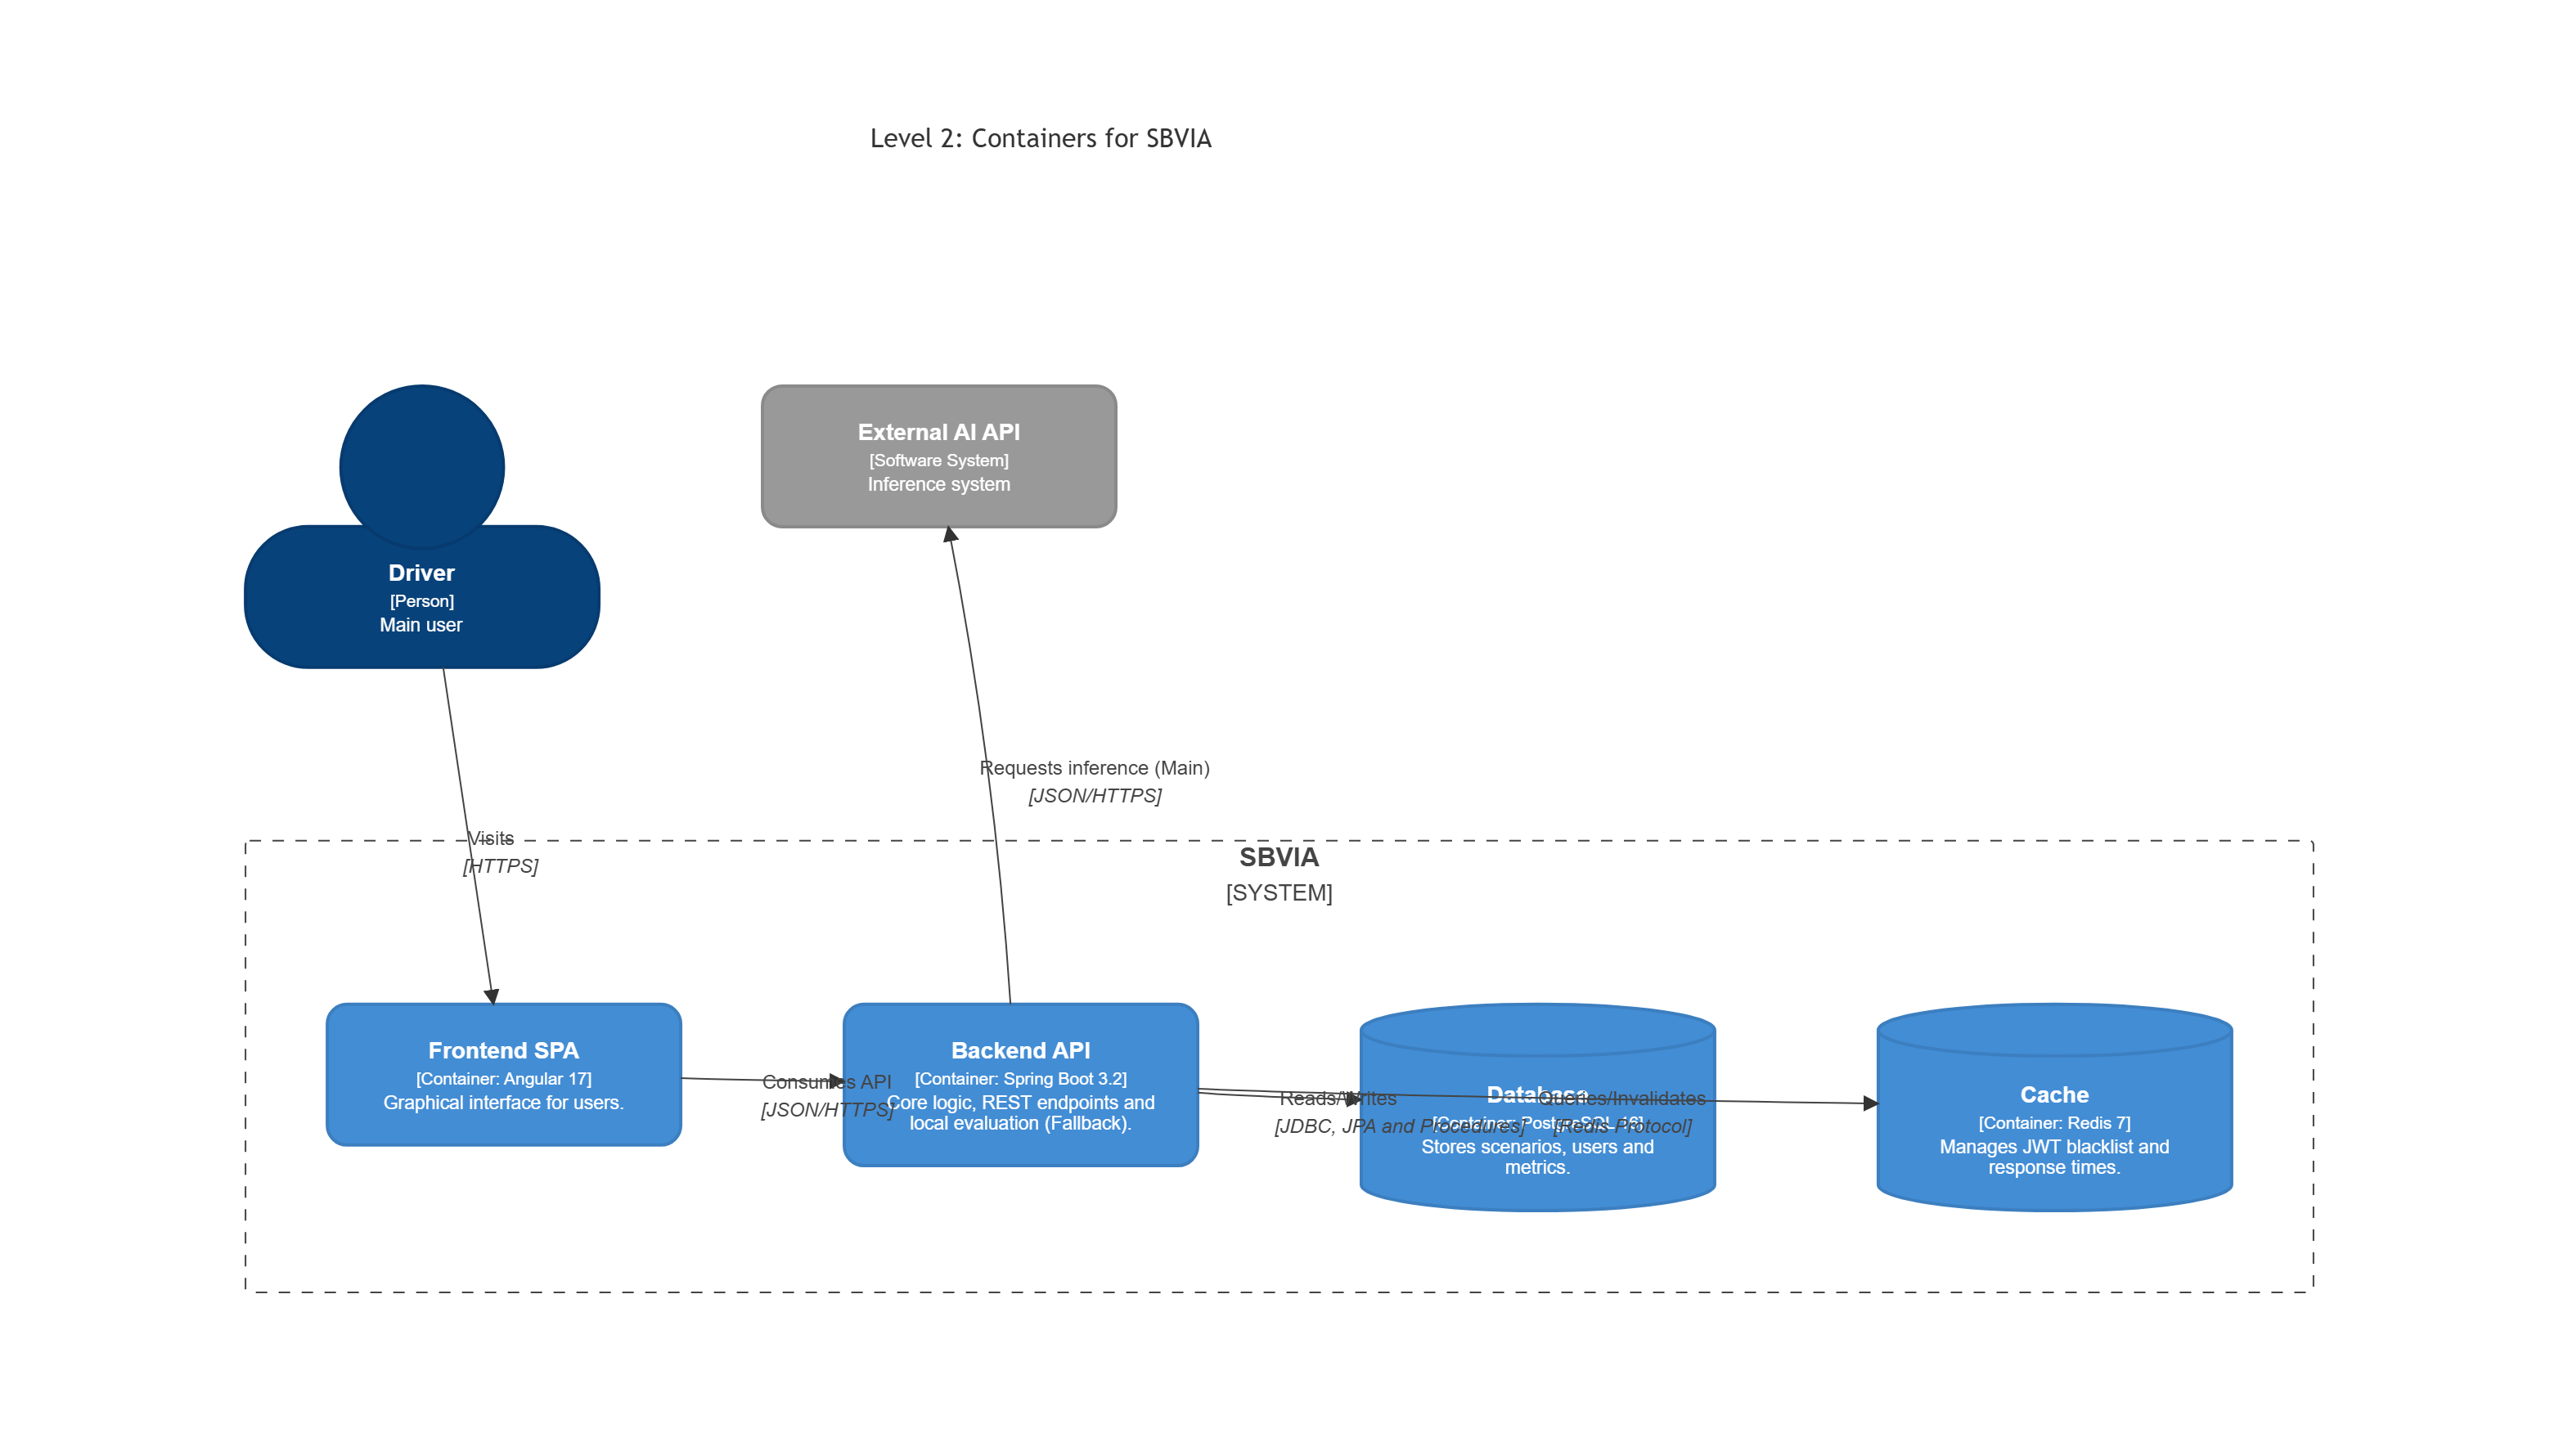
\includegraphics[width=0.95\textwidth]{diagramas/c4-level-2.png}
    \caption{C4 Container diagram (Level 2) for SBVIA. Source: Own elaboration.}
    \label{fig:c4-level2}
\end{figure}

\section{Estructura de Objetos del Dominio Central}
La orientación a objetos del núcleo del sistema aísla las reglas de negocio de los límites de infraestructura. Como se aprecia en la Figura~\ref{fig:uml-classes}, las abstracciones principales interactúan de forma segura durante una simulación.

\begin{figure}[htbp]
\centering
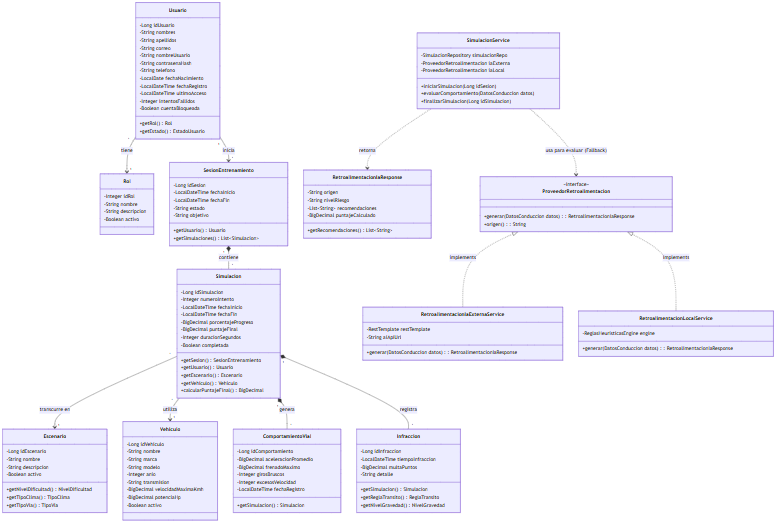
\includegraphics[width=0.7\textwidth]{diagramas/uml-classes-en.png}
\caption{UML class diagram of the main components. Source: Own elaboration.}
\label{fig:uml-classes}
\end{figure}

\section{Ingeniería de Usabilidad}
Para garantizar que las herramientas educativas sean accesibles e intuitivas para conductores novatos, las evaluaciones empíricas de usabilidad son imprescindibles. El Cuestionario de Usabilidad del Sistema (SUS) \cite{brooke1996sus} proporciona una métrica estandarizada para evaluar el desempeño interactivo.

% ==========================================
% B.6 CAPÍTULO 3: TRABAJOS RELACIONADOS
% ==========================================
\chapter{Trabajos Relacionados}
Se realizó una revisión narrativa estructurada tomando como referencia las directrices de Kitchenham \& Charters \cite{kitchenham2007guidelines} y PRISMA 2020 \cite{page2021prisma}. No se presenta como una revisión sistemática completa, porque el proyecto no conserva un protocolo registrado ni un conjunto íntegro de resultados de búsqueda y exclusión. La síntesis se limita a trabajos identificables y directamente relacionados con la eficacia o validez de simuladores de conducción.

\begin{table}[htbp]
\centering
\caption{Systematic comparison of related work against SBVIA}
\label{tab:trabajos_relacionados}
\footnotesize
\begin{tabularx}{\textwidth}{p{2.8cm}p{1cm}p{2.4cm}p{2.2cm}X}
\toprule
\textbf{Referencia} & \textbf{Año} & \textbf{Tipo} & \textbf{Corpus} & \textbf{Aporte y relación con SBVIA} \\
\midrule
Martín-delosReyes et al. \cite{martin2019simulator} & 2019 & Revisión sistemática & 5 estudios & Evidencia insuficiente y heterogénea; sustenta una interpretación conservadora del alcance formativo. \\
Wynne et al. \cite{wynne2019validation} & 2019 & Revisión de validación & 44 estudios & Aproximadamente la mitad mostró validez absoluta o relativa; diferencia entre desempeño simulado y real. \\
Alonso et al. \cite{alonso2023simulators} & 2023 & Revisión sistemática & 15 estudios & Reporta indicios favorables, pero advierte muestras limitadas y falta de seguimiento longitudinal. \\
Krasniuk et al. \cite{krasniuk2024simulator} & 2024 & Revisión de intervenciones & 15 estudios & Encuentra mejoras inmediatas en destrezas simuladas, sin certeza sobre transferencia duradera a carretera. \\
van Leeuwen et al. \cite{vanleeuwen2015changes} & 2015 & Estudio longitudinal breve & 52 novatos & Detecta cambios de control y mirada durante 30 minutos de práctica; orienta el registro de desempeño dentro de sesiones. \\
Rosenbloom y Eldror \cite{rosenbloom2014workshops} & 2014 & Estudio comparativo & 280 novatos & No encuentra una ventaja uniforme del entrenamiento simulado; justifica evitar afirmaciones causales fuertes. \\
Mayhew et al. \cite{mayhew2011validation} & 2011 & Validación concurrente & Conductores de 3 niveles & Encuentra concordancia relativa entre errores simulados y desempeño vial, pero no validez absoluta por tipo de error. \\
Hulme et al. \cite{hulme2021blueprint} & 2021 & Estudio de caso & Formación juvenil & Propone evaluación multimétrica de desempeño simulado; se relaciona con la combinación de métricas y retroalimentación de SBVIA. \\
\textbf{SBVIA} & \textbf{2026} & \textbf{Artefacto web} & \textbf{Caso académico} & \textbf{Integra escenarios, evaluación, trazabilidad y evidencia técnica reproducible; no mide reducción real de siniestros.} \\
\bottomrule
\end{tabularx}
\end{table}

\section{Brecha Identificada (Research Gap)}
La literatura revisada se concentra en el efecto pedagógico o en la validez del simulador, mientras que SBVIA aborda una brecha de ingeniería: documentar de forma trazable un artefacto web de apoyo formativo con autenticación, persistencia, caché, pruebas y mediciones reproducibles. Esta contribución es tecnológica y académica; los datos disponibles no permiten afirmar eficacia sobre la reducción de siniestros ni equivalencia con una práctica vial real.

% ==========================================
% B.6bis CAPÍTULO 4: INGENIERÍA DE REQUISITOS
% ==========================================
\chapter{Ingeniería de Requisitos}
\section{Interesados y Elicitación}
Se aplicó la técnica del *Stakeholder Onion* identificando usuarios directos (conductores en formación, instructores), operadores técnicos (administradores, DevOps) y entidades reguladoras (ANT/CTE).

Los conductores necesitan registrarse, autenticarse, consultar escenarios y recibir retroalimentación comprensible. Los administradores requieren gestionar catálogos y usuarios sin acceder a funciones fuera de su rol. El equipo técnico necesita diagnóstico, configuración reproducible y procedimientos de recuperación. Finalmente, el tribunal académico requiere trazabilidad entre requisito, implementación, prueba y evidencia. Estas perspectivas se documentaron mediante historias de usuario, casos de uso, matriz de trazabilidad y criterios de aceptación.

La elicitación combinó revisión del alcance académico, entrevistas semiestructuradas y análisis del sistema existente. Cada necesidad fue transformada en una declaración verificable, procurando que contuviera sujeto, obligación, acción, objeto y condición. La redacción normativa usa ``deberá'' para separar requisitos de explicaciones de diseño, de acuerdo con ISO/IEC/IEEE 29148 \cite{iso29148} y las prácticas de especificación de Wiegers y Beatty \cite{wiegers2013software}. Las historias siguen el enfoque de Cohn \cite{cohn2004user} y los casos de uso describen interacciones observables conforme a Cockburn \cite{cockburn2001writing}. La prioridad Must indica que el requisito es indispensable para la versión final; no implica que esté automáticamente verificado.

\section{Requisitos Funcionales y No Funcionales}
Los requisitos se redactaron según la plantilla sintáctica normativa de ISO/IEC/IEEE 29148:2018:
\begin{itemize}
    \item \textbf{RF-01 (Must):} El sistema deberá autenticar a los conductores mediante JWT firmado en cookie segura.
    \item \textbf{RF-02 (Must):} El sistema deberá gestionar el ciclo de vida completo de los escenarios viales (CRUD).
    \item \textbf{RF-03 (Must):} El sistema deberá consultar resultados consolidados multi-tabla mediante el procedimiento \texttt{sp\_reporte\_simulacion}.
    \item \textbf{RF-04 (Must):} El sistema deberá calcular el puntaje agregado del conductor vía \texttt{sp\_calcular\_promedio\_usuario}.
    \item \textbf{RNF-01 (Must):} La latencia de lectura con caché caliente deberá mantener un $p95 \le 200\text{ ms}$ con 50 VUs concurrentes.
    \item \textbf{RNF-03 (Must):} Las contraseñas deberán almacenarse hasheadas con algoritmo BCrypt.
\end{itemize}

\section{Alcance y exclusiones}
La versión evaluada cubre autenticación, roles, gestión de escenarios, registro de simulaciones, consulta de métricas y operaciones administrativas. El término ``simulador'' describe un flujo web de decisiones sobre escenarios viales; no representa un gemelo físico del vehículo ni reproduce fuerzas, campo visual o dinámica vehicular con fidelidad certificada. Tampoco realiza diagnóstico médico, evaluación legal de aptitud para conducir ni emisión de licencias.

Las capacidades de inteligencia artificial adaptativa, gráficos tridimensionales avanzados, integración con volante y telemetría en tiempo real se mantienen fuera del alcance de v1.0.0. Declarar estas exclusiones previene que funcionalidades futuras sean contabilizadasí como resultados presentes y permite evaluar el artefacto contra un límite funcional concreto.

\section{Trazabilidad y control de cambios}
La matriz ubicada en \texttt{docs/trazabilidad/matriz.csv} enlaza cada identificador con módulo, prueba, estado y tipo de acceso a datos. Los estados \texttt{VERIFIED}, \texttt{TESTED} y \texttt{PARTIAL} tienen significados distintos: verificado implica evidencia suficiente frente al criterio; probado indica que existe una comprobación automatizada del comportamiento referido; parcial señala que la evidencia o la implementación todavía no cubre el criterio completo.

El historial de requisitos registra adiciones y modificaciones entre entregas. Este mecanismo permite distinguir evolución legítima de alcance frente a regresiones. Una actualización de requisito debe reflejarse en su prueba, documentación y, cuando corresponda, decisión arquitectónica. De igual forma, una medición nueva no modifica por sí sola el requisito: únicamente actualiza su evidencia y estado de cumplimiento.

\section{Métricas de Calidad de Requisitos}
La tasa de estabilidad de requisitos calculada es:
\begin{equation}
    T_{est} = 1 - \frac{N_{mod}}{N_{total}} = 1 - \frac{2}{20} = 0.90 \quad (90\%)
\end{equation}
La matriz registra 12 de 14 requisitos \emph{Must} como verificados ($85.71\%$). RNF-01 y RNF-02 conservan estado parcial hasta completar las cinco corridas y la comparación homogénea de caché fría y caliente.

% ==========================================
% B.7 CAPÍTULO 5: MATERIALES Y MÉTODOS
% ==========================================
\chapter{Materiales y Métodos}
\section{Enfoque Metodológico (DSR de Peffers)}
Se adoptó la metodología Design Science Research \cite{peffers2007design, hevner2004design} estructurada en 6 actividades:
1) Identificación del problema, 2) Definición de objetivos, 3) Diseño y desarrollo, 4) Demostración, 5) Evaluación empírica y 6) Comunicación.

Las preguntas y métricas se relacionaron mediante Goal--Question--Metric \cite{basili1994gqm}, como se detalla en la Tabla \ref{tab:gqm}. El diseño de las mediciones siguió principios de experimentación en ingeniería de software \cite{wohlin2012experimentation}; la selección por conveniencia de participantes se declara explícitamente porque este tipo de muestreo limita la generalización \cite{baltes2022sampling}.

\begin{table}[htbp]
\centering
\caption{Application of the Goal-Question-Metric (GQM) approach to the SBVIA evaluation}
\label{tab:gqm}
\footnotesize
\begin{tabularx}{\textwidth}{p{3.5cm}Xp{2.5cm}p{2.5cm}}
\toprule
\textbf{Goal (Objetivo)} & \textbf{Question (Pregunta)} & \textbf{Metric (Métrica)} & \textbf{Source/Tool} \\
\midrule
\textbf{G1. Rendimiento:} Evaluar la capacidad de respuesta bajo carga concurrente & ¿El sistema responde de manera oportuna a 50 usuarios simultáneos? & Latencia percentil 95 ($p95 \le 200$ ms) y tasa de error & k6 \\
\midrule
\textbf{G2. Usabilidad:} Medir la facilidad de uso percibida del prototipo & ¿Es el sistema considerado usable por los conductores novatos? & Puntuación individual y media SUS (umbral $\geq$ 68). \textbf{Media 69,00; DE 9,90; IC 95\,\% [63,52; 74,48]} & Cuestionario SUS de Brooke, aplicado ($N = 15$) \\
\midrule
\textbf{G3. Seguridad:} Comprobar la resiliencia contra ataques comunes & ¿El backend implementa cabeceras seguras y carece de defectos críticos? & Número de hallazgos por severidad; controles de cabeceras & OWASP ZAP, SpotBugs, \texttt{curl} \\
\midrule
\textbf{G4. Calidad Web:} Auditar las mejores prácticas en el frontend & ¿El frontend cumple con estándares de accesibilidad y SEO? & Puntajes de 0 a 100 en Performance, Accessibility, Best Practices, SEO & Lighthouse CI \\
\midrule
\textbf{G5. Calidad Interna:} Verificar la suficiencia de las pruebas automatizadas & ¿Qué proporción del código fuente está cubierta por pruebas unitarias? & Porcentaje de cobertura de líneas y de ramas ($\ge 70\%$) & JaCoCo \\
\midrule
\textbf{G6. Reproducibilidad:} Garantizar que la evidencia sea auditable & ¿Los datos y procedimientos cumplen lineamientos científicos de apertura? & Cumplimiento de artefactos (proveniencia, datos crudos) & Checklists FAIR y Ralph \\
\bottomrule
\end{tabularx}
\end{table}

\section{Instrumentos de Medición y Protocolo Experimental}
\begin{itemize}
    \item \textbf{Rendimiento:} k6 (50 VUs / 30s) en 5 corridas independientes de caché caliente y una medición complementaria de 10 ciclos frío/caliente.
    \item \textbf{Usabilidad:} Cuestionario SUS de 10 ítems \cite{brooke1996sus} con $N = 15$ respuestas registradas. La reevaluación de septiembre de 2026 alcanzó una media de \textbf{69,00}, que cumple el criterio de $RNF\text{-}06$ (véase la sección de Usabilidad); el estudio de julio de 2026 permanece retirado.
    \item \textbf{Seguridad:} Script reproducible de curl, escaneo OWASP ZAP 2.14 y análisis estático SpotBugs 4.8.
    \item \textbf{Calidad Web:} Auditoría Lighthouse CI (mobile/desktop).
    \item \textbf{Cobertura:} JaCoCo 0.8.12 sobre capas de servicio, controlador y dominio.
\end{itemize}

\section{Población, muestra y estrategia de muestreo}
La población objetivo de la evaluación de usabilidad corresponde a conductores en formación capaces de utilizar un navegador web moderno. La unidad de análisis es el individuo (conductor). El contexto de aplicación es un entorno académico controlado donde el usuario interactúa con los módulos del simulador web a través del prototipo desplegado.

La muestra disponible comprende 15 participantes, identificados exclusivamente mediante los códigos P01--P15. La selección fue no probabilística por conveniencia: se invitó a personas accesibles para el equipo dentro del contexto académico. Este procedimiento permite una evaluación formativa del prototipo, pero introduce sesgo de selección y no garantiza representatividad por edad, experiencia vial, ubicación geográfica o familiaridad tecnológica \cite{baltes2022sampling}.

En consecuencia, los resultados SUS describen únicamente a la muestra observada. No se extrapolan a la población nacional de conductores ni se interpretan como evidencia empírica de reducción de siniestros. Los archivos públicos no incluyen edad, género, dispositivo ni otros atributos demográficos; por ello, el informe tampoco afirma diversidad sobre variables que no fueron estrictamente registradas.

\section{Preguntas, hipótesis y análisis estadístico}
La evaluación cuantitativa se organiza con un nivel de significación $\alpha=0.05$. Para rendimiento, la hipótesis nula es $H_{0R}$: la latencia $p95$ de lecturas frías no es mayor que la de lecturas calientes bajo el mismo perfil; la alternativa unilateral $H_{1R}$ establece que la latencia fría es mayor. Cuando existan cinco pares homogéneos se aplicará Wilcoxon de rangos con signo, se informará el valor $p$ en notación científica y se acompañará con $A_{12}$ de Vargha--Delaney o delta de Cliff \cite{arcuri2012hitchhiker,vargha2000critique,cliff1993dominance}. No se emitirá una conclusión inferencial mientras falten esos pares.

Para usabilidad se declaró $H_{0U}$: la media poblacional SUS no supera el umbral de 68, frente a $H_{1U}$, que lo supera. \textbf{El contraste se resuelve con la reevaluación de septiembre de 2026}: la media observada es \textbf{69,00} y su intervalo de confianza al 95\,\% es [63,52; 74,48], que incluye el umbral, de modo que \textbf{no se rechaza $H_{0U}$} al 5\,\%. El criterio de aceptación de $RNF\text{-}06$ —media muestral igual o superior a 68 con al menos 15 participantes— sí se cumple, con un margen de $+1,00$. El estudio de julio de 2026 permanece retirado. Para cobertura, seguridad y Lighthouse se aplican criterios de aceptación previamente fijados y no pruebas de hipótesis retrospectivas.

La familia de hipótesis se declaró contemplando dos pruebas sobre el mismo experimento (rendimiento frío/caliente y usabilidad SUS frente al umbral de 68). Al sustituirse la evidencia retirada por la reevaluación de septiembre, en este informe permanecen evaluables la comparación de rendimiento y el contraste de usabilidad frente al umbral; el procedimiento de Holm-Bonferroni se mantiene documentado para el caso en que se incorporen nuevas pruebas. De aplicarse, los valores $p$ obtenidos se ordenarían de menor a mayor y se compararían contra niveles de significancia ajustados progresivamente ($\alpha / k, \alpha / (k-1), \dots$) antes de rechazar cualquier hipótesis nula \cite{holm1979simple}.

\section{Variables y criterios de aceptación}
Para rendimiento, la variable principal es la duración de solicitudes HTTP y el estadístico de decisión es el percentil 95. Se selecciona $p95$ porque representa el límite experimentado por la mayoría de usuarios sin ocultar la cola de latencias tras una media. Las variables secundarias son $p50$, $p90$, $p99$, media, desviación y tasa de errores. Los criterios son $p95 \le 200$ ms con caché caliente y $p95 \le 500$ ms en frío.

Para cobertura, las unidades son líneas y ramas instrumentadas por JaCoCo. La cobertura de líneas confirma ejecución, mientras que la de ramas exige recorrer resultados alternativos de decisiones. Ambas deben alcanzar al menos 70\%; aprobar solo una no satisface el criterio conjunto. Para usabilidad, la variable declarada fue el puntaje SUS individual en escala de 0 a 100 y el umbral del proyecto 68, pero el estudio se retira y esa variable no se analiza. Para seguridad, se utilizan resultados categóricos por control, hallazgos del escáner y ausencia de defectos de severidad bloqueante.

\section{Procedimiento reproducible}
El protocolo comienza desde una copia limpia del repositorio. Se configuran las variables descritas en \texttt{.env.example}, se construyen los contenedores y se espera a que los chequeos de salud confirmen PostgreSQL, Redis, backend y frontend. Las pruebas unitarias se ejecutan antes de carga para evitar medir una versión funcionalmente defectuosa. Cada corrida de rendimiento conserva su salida cruda y un resumen tabular con identificador, carga, duración y percentiles.

La condición fría requiere invalidar Redis antes de la lectura inicial; la condición caliente requiere precargar la misma clave y mantener constantes endpoint, conjunto de datos, número de usuarios virtuales y duración. Las corridas deben alternarse o parearse para reducir el sesgo temporal. El análisis estadístico solo se calcula cuando se dispone de al menos cinco pares comparables. Lighthouse se ejecuta sobre una compilación de producción, y los controles de seguridad se aplican contra servicios levantados con configuración equivalente a la documentada.

Para SUS, el protocolo declarado preveía que cada participante completara una sesión guiada y respondiera inmediatamente los diez ítems estándar en escala Likert de 1 a 5; los ítems impares aportan $respuesta-1$ y los pares $5-respuesta$, y la suma se multiplica por 2.5. \textbf{Ese protocolo no puede sostenerse contra el historial del repositorio} (véase la sección de Usabilidad): la fecha declarada de aplicación es anterior a la existencia de la funcionalidad de simulación. El archivo crudo se conserva como material sin garantía de validez metodológica.

Las herramientas declaradas corresponden a las configuraciones versionadas: JaCoCo 0.8.12, SpotBugs 4.8 con FindSecBugs, OWASP ZAP 2.14, Angular 17 y el JSON de Lighthouse conserva su propia versión y fecha. Los comandos exactos, entradas crudas y productos se relacionan en \texttt{DATA-PROVENANCE.md} para evitar atribuir a una herramienta resultados redactados manualmente.

\section{Gestión de evidencia}
Los archivos crudos no se reemplazan por capturas aisladas. Los JSON de k6 y Lighthouse permiten recalcular indicadores; los CSV facilitan inspección; y los documentos Markdown explican comandos, ambiente y decisiones. \texttt{DATA-PROVENANCE.md} relaciona datos con scripts, mientras \texttt{DATA-DICTIONARY.md} define columnas y unidades. Esta separación entre dato, transformación e interpretación sigue las recomendaciones para investigación reproducible \cite{sandve2013ten, ralph2021empirical}.

\section{Integridad de datos y evidencia retractada}
\label{sec:retractaciones}
Este informe declara qué evidencia fue retractada y por qué. El registro completo, con el commit exacto de cada corrección, se mantiene en \texttt{docs/RETRACTIONS.md} y abarca catorce retractaciones: los JSON de Lighthouse escritos a mano (\texttt{fc4c701}); el \texttt{report.json} fabricado y las cifras de una corrida local presentadas como producción (\texttt{2ad52ff}, \texttt{5fa54d6}); la salida de \texttt{grep} no reproducible del expediente (\texttt{e7a1e34}); los p-valores fijados a mano en lugar de calculados (\texttt{7b3cfbe}); los DOI que apuntaban a obras distintas de las citadas (\texttt{94fdd61}); la lista blanca de fallos del verificador (\texttt{7a691d0}); el estudio SUS retirado por incompatibilidad con el historial del repositorio (\texttt{ec56c20}, \texttt{93ab5ce}); la corrección de una migración ya aplicada (\texttt{deda187}); una atribución al docente-director sin texto que la respaldara (\texttt{5c02c22}); cuatro citas a un informe de revisión que no existía en el repositorio (\texttt{5c02c22}); una autorización del docente-director fechada el 19 de septiembre cuando consta por escrito el 20, en dos archivos (\texttt{R-11}); la anterioridad del instrumento de usabilidad afirmada en cinco archivos, con una primera corrección que dejó dos a medias (\texttt{R-12}); una cifra falsa sobre el renombrado en el mensaje de un commit, repetida en dos rondas (\texttt{R-13}); y la versión del esquema de citación rota por un reemplazo global de texto (\texttt{R-14}).

Estas retractaciones corrigen la evidencia del expediente, no el resultado de los puntos afectados: RNF-06 pasa a \texttt{VERIFIED} con la reevaluación de septiembre, RNF-02 declara su umbral incumplido con la medición real, y RF-16 a RF-20 pasan a \texttt{NOT VERIFIED} porque sus procedimientos no se invocan desde la aplicación. Se documentan aquí porque la magnitud de lo corregido obliga a una lectura cuidadosa del informe, y esa lectura solo es posible si el propio informe dice qué se retiró y por qué.

% ==========================================
% B.8 CAPÍTULO 6: DISEÑO DEL SISTEMA Y ARQUITECTURA
% ==========================================
\chapter{Diseño del Sistema y Arquitectura}
\section{Modelo Arquitectónico C4}
El sistema se modeló en niveles 1 (Contexto), 2 (Contenedores) y 3 (Componentes) utilizando Structurizr DSL. El backend en Spring Boot desacopla las responsabilidades en capas de Controlador, Servicio, Repositorio y Seguridad.

En el nivel de contexto (ver Figura~\ref{fig:c4-level1}), el conductor y el administrador acceden mediante navegador, mientras los servicios de persistencia permanecen aislados de Internet. En el nivel de contenedores, Angular entrega la interfaz, Spring Boot expone la API, PostgreSQL conserva el estado durable y Redis almacena datos temporales. Docker Compose define red, dependencias y verificaciones de salud. 

El \textbf{Diagrama de Contexto (Nivel 1)} proporciona una visión general de las interacciones entre los usuarios (Estudiante, Instructor, Administrador) y el Sistema SBVIA, así como las dependencias externas.
\begin{figure}[htbp]
    \centering
    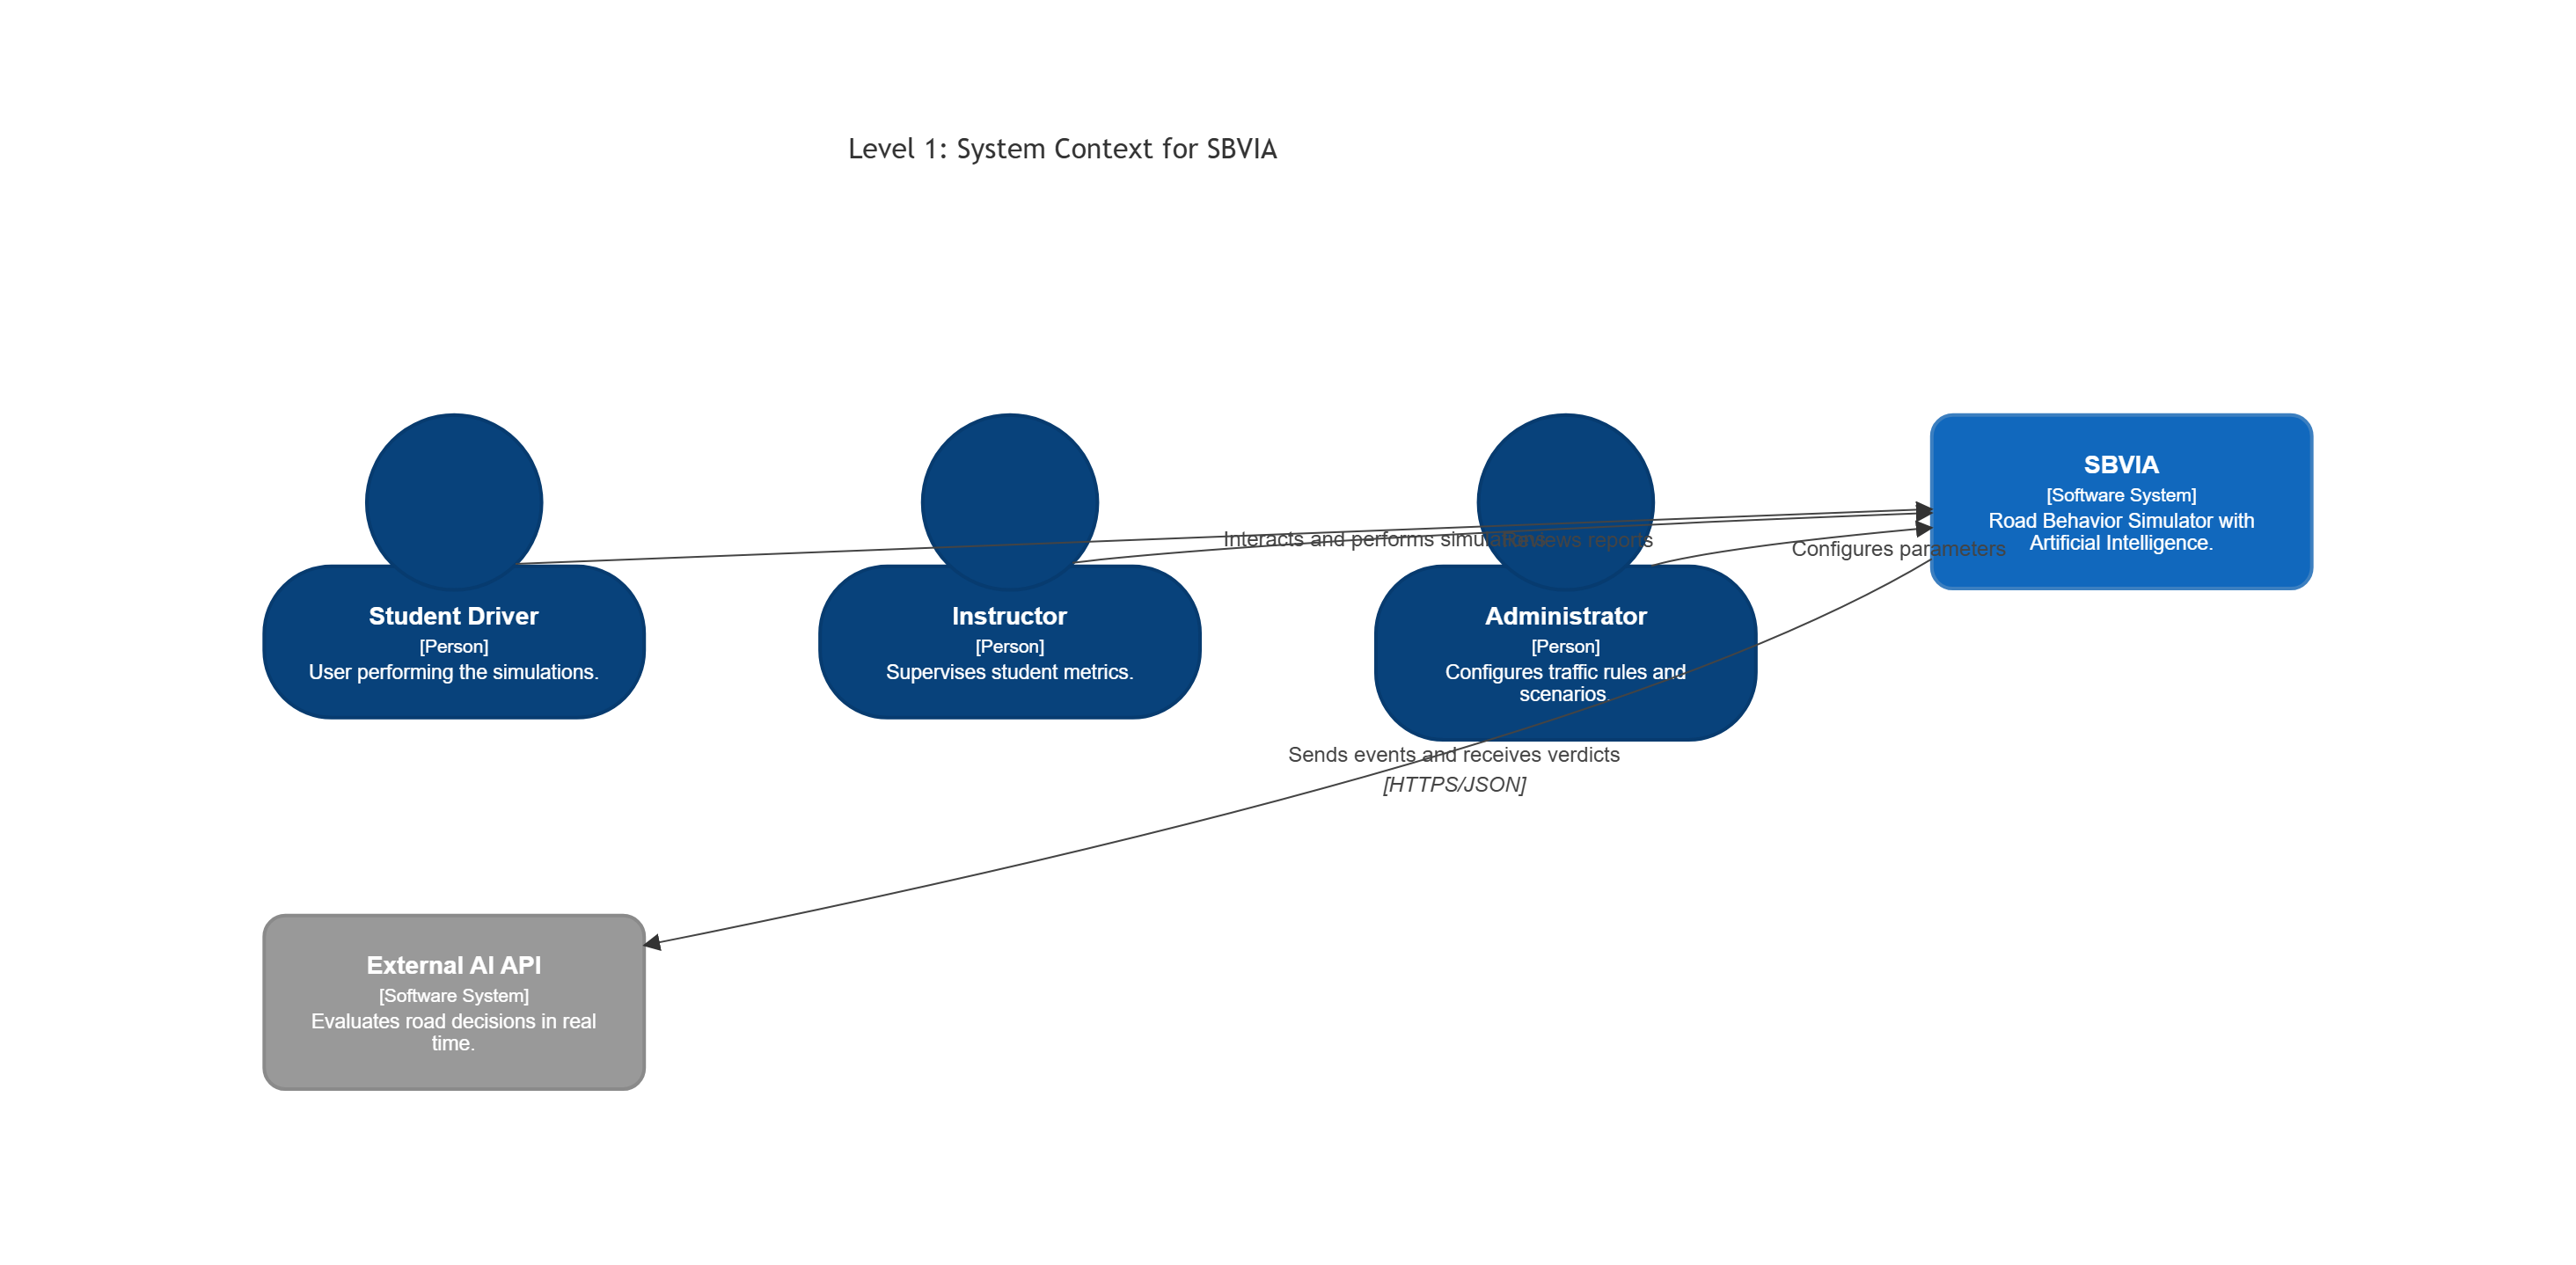
\includegraphics[width=0.95\textwidth]{diagramas/c4-level-1.png}
    \caption{C4 Context diagram (Level 1) for SBVIA. Source: Own elaboration.}
    \label{fig:c4-level1}
\end{figure}

En el nivel de componentes (ver Figura~\ref{fig:c4-level3}), los controladores traducen HTTP, los servicios aplican reglas, los repositorios abstraen persistencia y la configuración de seguridad forma la frontera de confianza.

El \textbf{Diagrama de Componentes (Nivel 3)} se enfoca en el backend de Spring Boot, ilustrando los controladores, servicios y repositorios clave que manejan la lógica de negocio (Simulaciones, Autenticación, Reportes).
\begin{figure}[htbp]
    \centering
    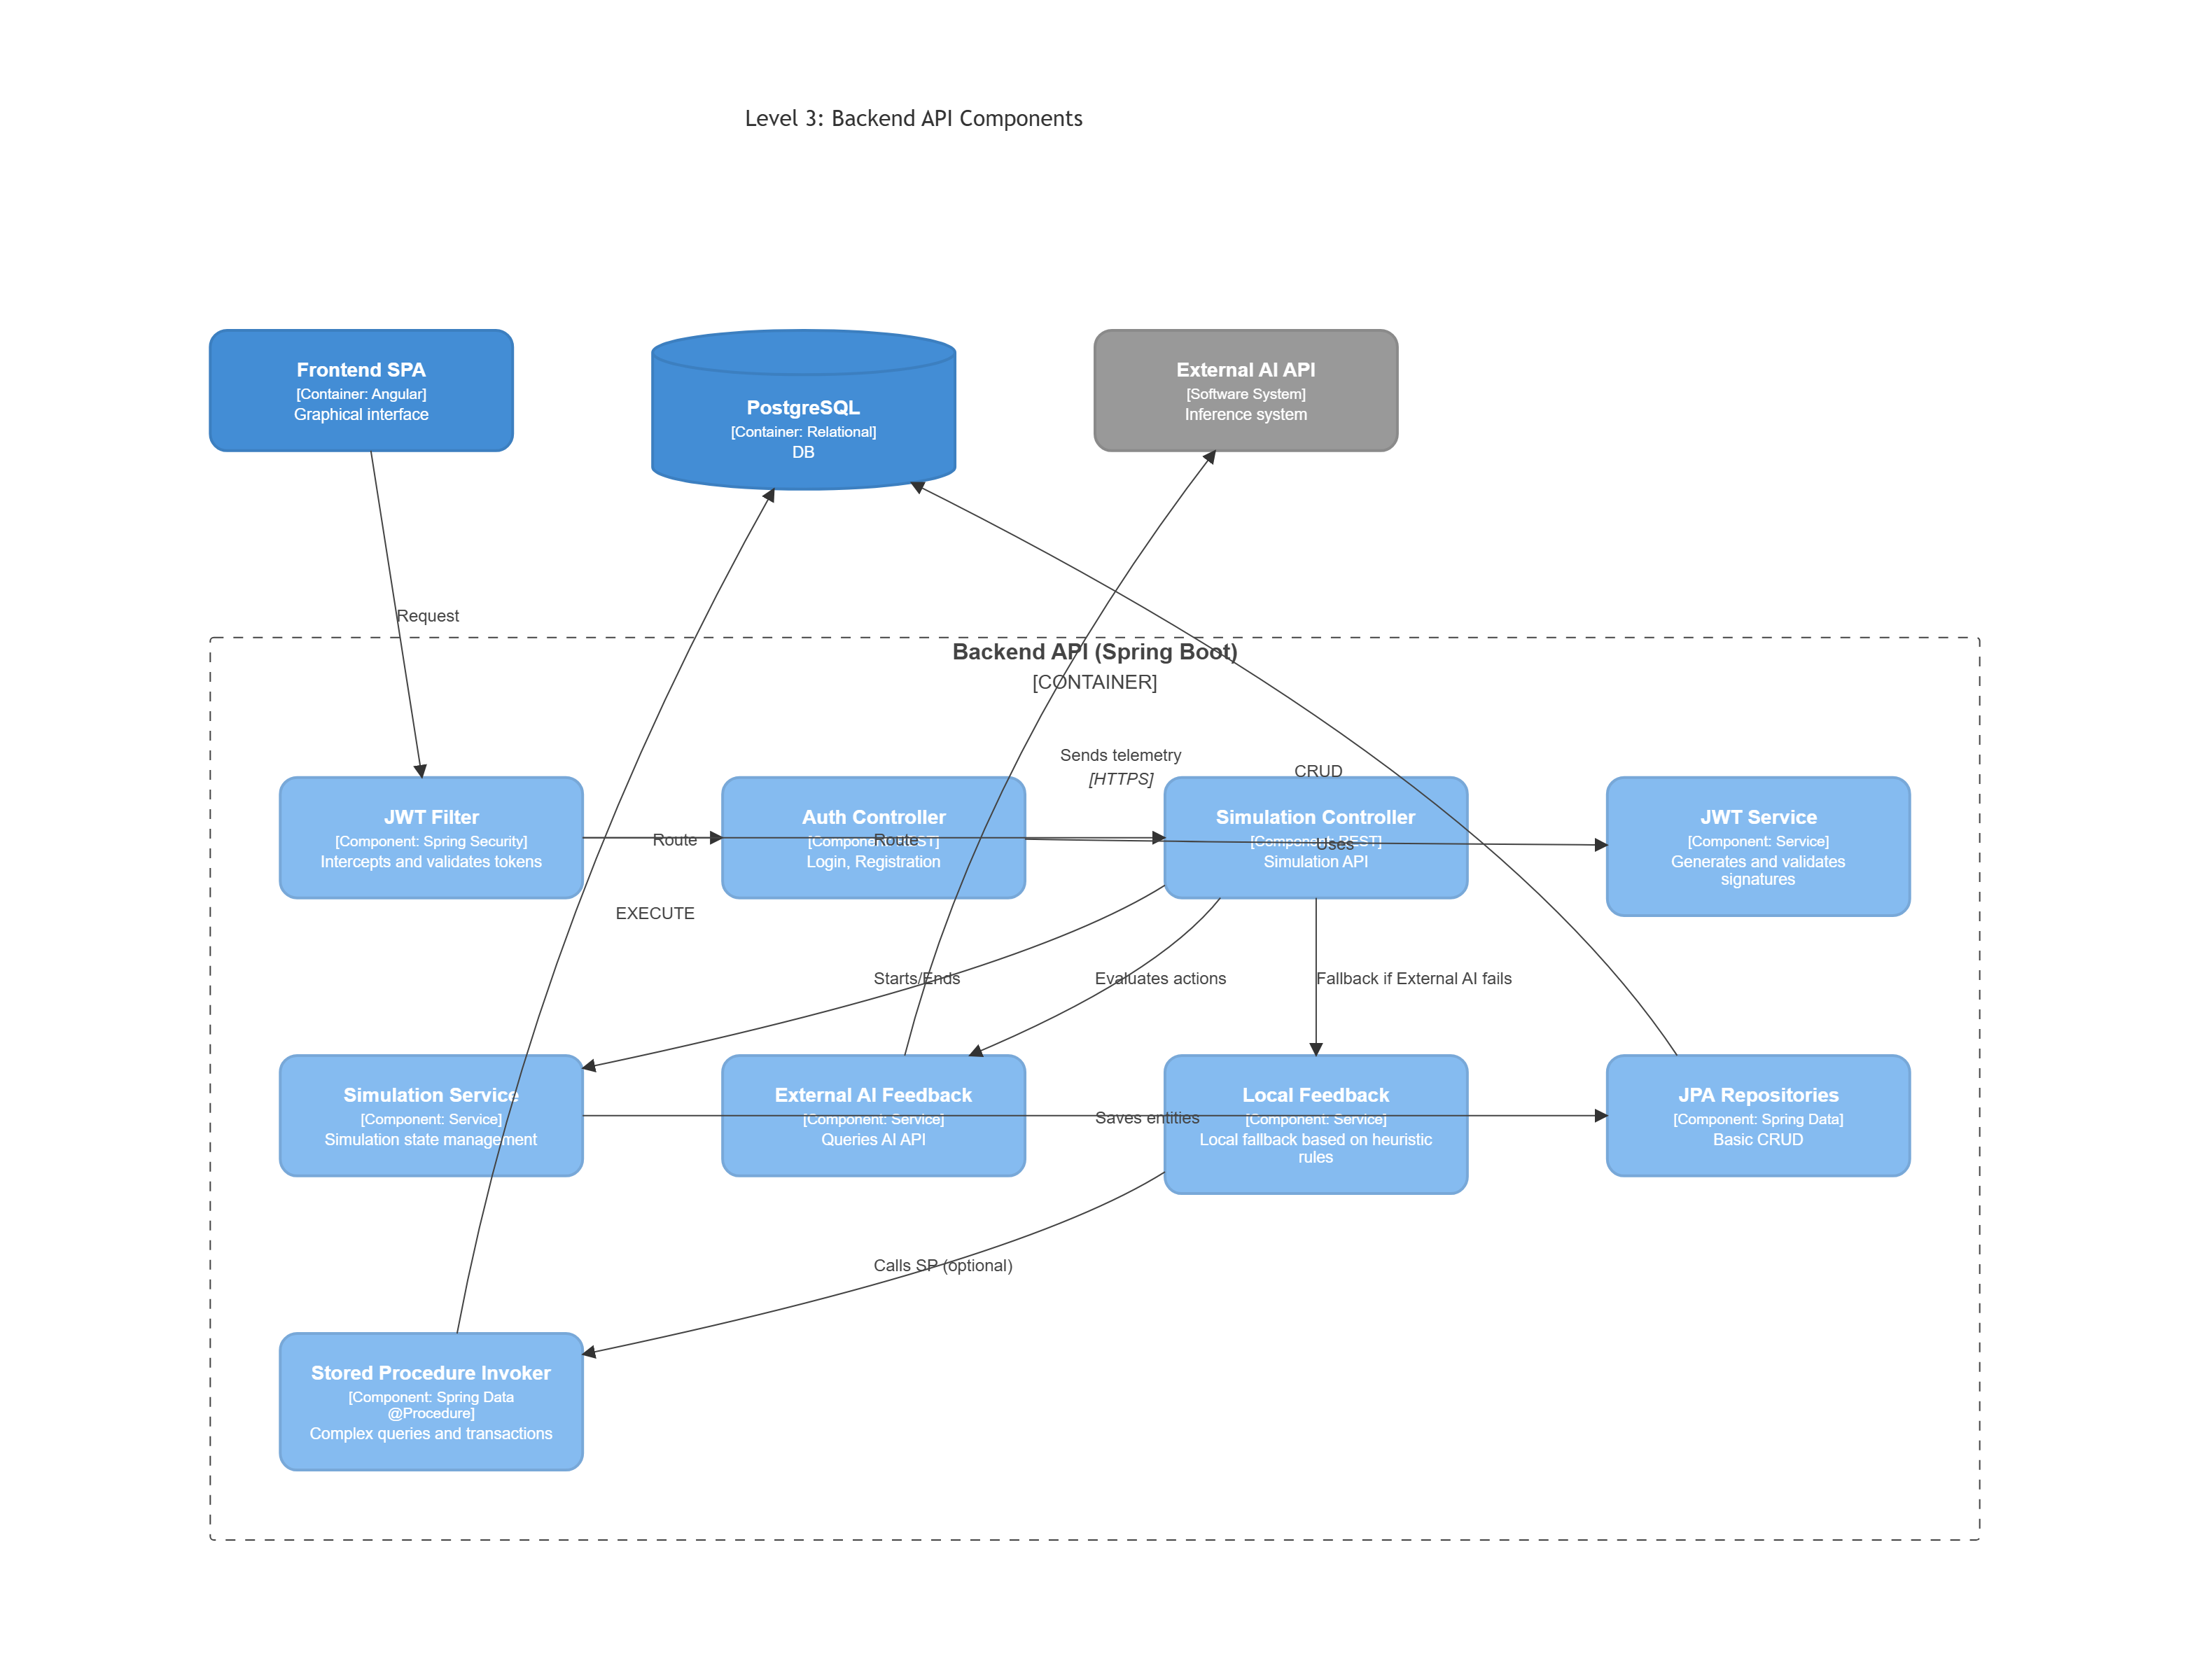
\includegraphics[width=0.95\textwidth]{diagramas/c4-level-3.png}
    \caption{C4 Component diagram (Level 3) for the backend. Source: Own elaboration.}
    \label{fig:c4-level3}
\end{figure}

La API adopta las restricciones de interfaz uniforme y comunicación sin estado asociadas al estilo REST \cite{fielding2000architectural}. Spring Boot proporciona la composición de componentes, configuración y acceso HTTP usados por el backend \cite{walls2022spring}; estas tecnologías se documentan como decisiones de implementación y no como evidencia de calidad por sí mismas.

El recorrido típico comienza con una petición HTTPS al frontend. La aplicación envía solicitudes a la API incluyendo credenciales según la política de cookies. El filtro de seguridad valida sesión y rol antes de invocar el controlador. Para una consulta de escenarios, el servicio intenta recuperar la representación serializada desde Redis; si no existe, consulta PostgreSQL, construye la respuesta y actualiza la caché. En una modificación, el servicio persiste y debe invalidar las entradas relacionadas para evitar servir datos obsoletos.

As shown in Figure~\ref{fig:flujo-mvc}, la separación mostrada permite ubicar la validación HTTP en el controlador, las reglas en el servicio y el acceso durable en los repositorios, evitando que la interfaz dependa directamente del motor de datos.

\subsection{Flujo de Interacción MVC}
El patrón Modelo-Vista-Controlador (MVC) dicta cómo fluye la información a través de la aplicación. La Figura~\ref{fig:flujo-mvc} ilustra este flujo en el entorno Spring Boot: las peticiones HTTP del cliente son recibidas por el Controlador, el cual delega la lógica al Servicio. El Servicio manipula el Modelo y los DTOs interactuando con la base de datos a través de los Repositorios. Finalmente, la respuesta viaja de vuelta al cliente.

\begin{figure}[htbp]
    \centering
    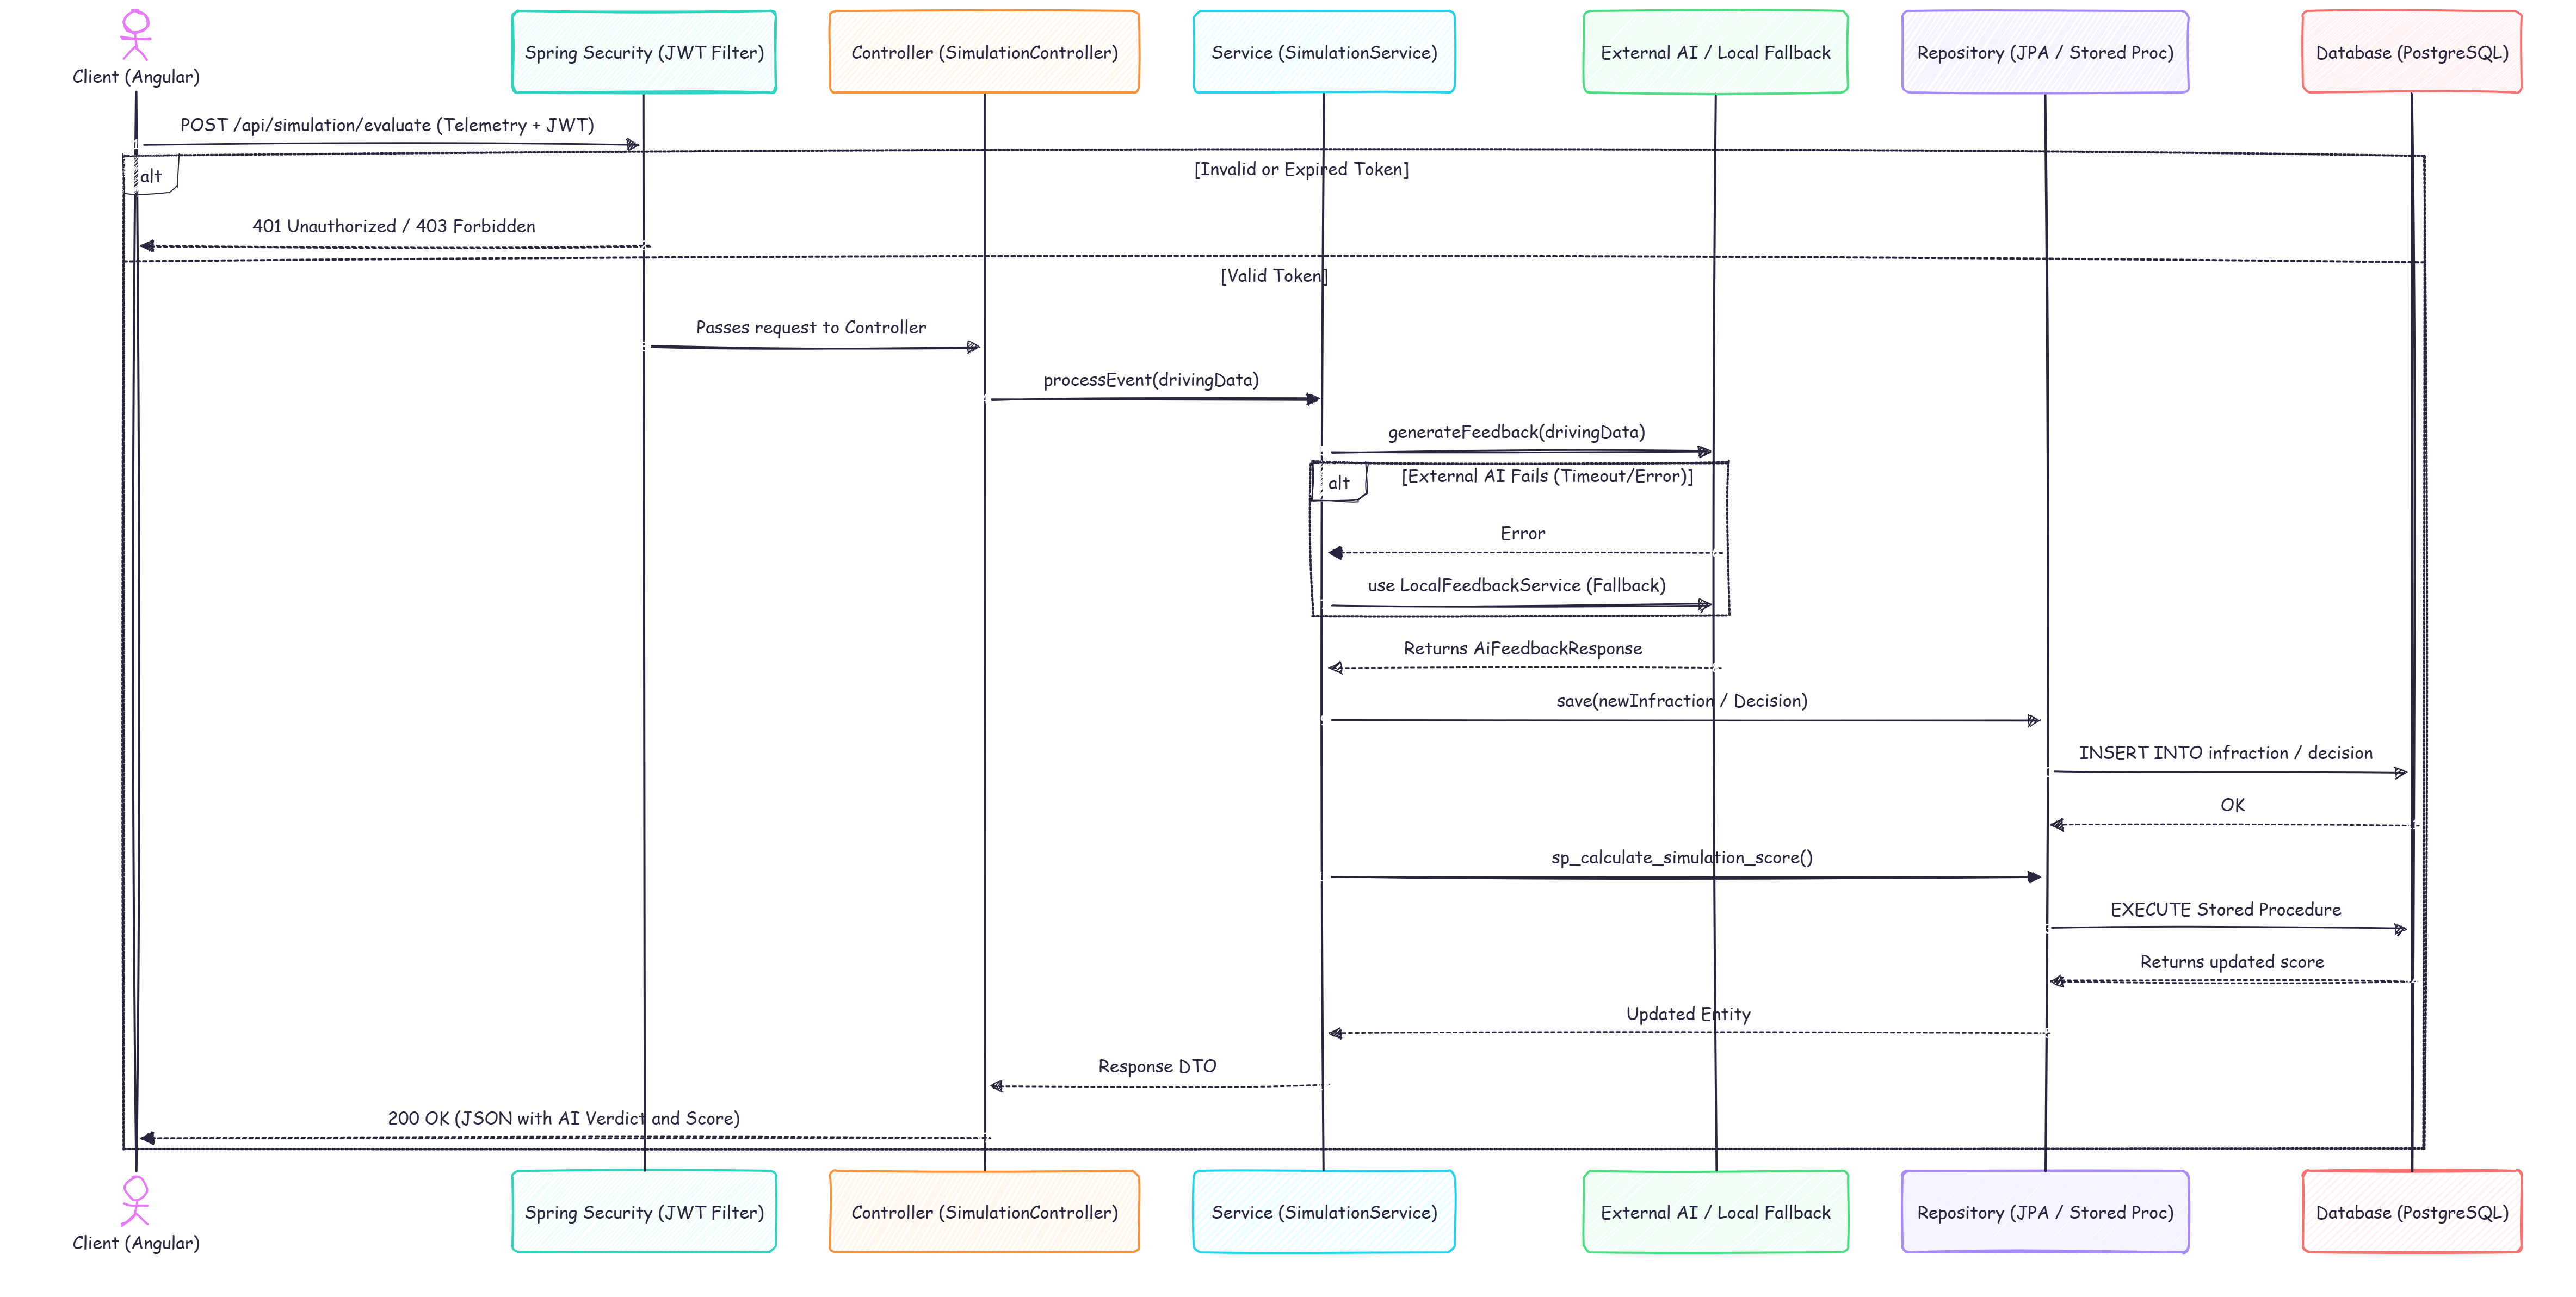
\includegraphics[width=0.95\textwidth]{diagramas/mvc-flow-springboot-en.png}
    \caption{MVC data flow between Angular, Spring Boot, Redis and PostgreSQL. Source: Own elaboration from SBVIA versioned architecture.}
    \label{fig:flujo-mvc}
\end{figure}

\section{Atributos arquitectónicos}
La seguridad se favorece mediante mínimo privilegio, separación de roles y secretos externos a la imagen. La mantenibilidad se apoya en dependencias dirigidas y responsabilidades diferenciadas. La portabilidad proviene de imágenes reproducibles y configuración por variables. La observabilidad usa endpoints de salud y registros de eventos. La escalabilidad horizontal es viable para el backend si el estado compartido permanece en PostgreSQL y Redis; cualquier dato de sesión almacenado solo en memoria de una instancia limitaría esa propiedad \cite{bass2021software, richards2020fundamentals}.

La arquitectura también tiene compromisos. Redis añade complejidad operativa y posibles problemas de consistencia; los procedimientos almacenados aumentan dependencia con PostgreSQL; y JWT exige revocación y rotación bien definidas. Los ADR documentan estas decisiones para que una alternativa futura pueda evaluarse contra el contexto original, no únicamente contra preferencias tecnológicas.

\section{Registros de Decisión Arquitectónica (ADRs)}
Se formalizaron 7 ADRs bajo la plantilla de Nygard:
\begin{enumerate}
    \item \textbf{ADR-001:} Elección de la pila tecnológica (Spring Boot 3.2 + Angular 17).
    \item \textbf{ADR-002:} Migración y compatibilidad con Java 21 LTS.
    \item \textbf{ADR-003:} Autenticación stateless con JWT y cookies seguras.
    \item \textbf{ADR-004:} Estrategia de caché distribuida con Redis 7.
    \item \textbf{ADR-005:} Mitigación de riesgos de seguridad OWASP Top 10.
    \item \textbf{ADR-006:} Estrategia híbrida de acceso a datos (Separación CRUD / SP).
    \item \textbf{ADR-007:} Estrategia de despliegue en contenedores orquestados con HTTPS.
\end{enumerate}

ADR-008 documenta posteriormente la comparación Angular frente a React. Esta adición no invalida ADR-001: amplía su justificación con criterios de estructura, experiencia del equipo, ecosistema y costo de migración. En conjunto, los ADR constituyen una memoria de decisiones; no son manuales de implementación ni sustituyen pruebas.

% ==========================================
% B.9 CAPÍTULO 7: IMPLEMENTACIÓN
% ==========================================
\chapter{Implementación}
\section{Estrategia Híbrida de Acceso a Datos}
Siguiendo las recomendaciones de OWASP para la prevención de SQL Injection \cite{owasp2021}, las operaciones analíticas se encapsularon en procedimientos almacenados PostgreSQL en `db/procs/`.

El catálogo identifica seis procedimientos exigidos por la entrega: reporte de simulación, promedio por usuario, reporte diario, actualización de inactivos, validación de escenario y generación de código de certificado. Cada entrada registra propósito, parámetros, tablas involucradas y consumidor previsto. Las migraciones Flyway mantienen el esquema bajo control de versiones y permiten reconstruir una base vacía en el mismo orden.

El uso de parámetros evita concatenar entrada del usuario dentro de SQL. No obstante, un procedimiento almacenado no es seguro por definición: también requiere privilegios mínimos, validación de argumentos y revisión de cualquier sentencia dinámica. Por ello, el repositorio incluye una auditoría estática específica y pruebas de integración sobre repositorios.

\begin{lstlisting}[language=SQL, caption={Procedimiento almacenado para reporte multi-tabla (sp\_reporte\_simulacion.sql)}]
CREATE OR REPLACE FUNCTION sp_reporte_simulacion(p_id_simulacion INTEGER)
RETURNS TABLE (
    simulacion_id INTEGER,
    usuario_nombre VARCHAR,
    escenario_nombre VARCHAR,
    puntaje_final DECIMAL,
    estado_simulacion VARCHAR,
    tiempo_reaccion DECIMAL
) AS $$
BEGIN
    RETURN QUERY
    SELECT s."id_Simulacion", u."nombre", e."nombre", s."puntaje_final", s."estado", m."tiempo_reaccion"
    FROM "Simulacion" s
    INNER JOIN "Usuario" u ON s."id_Usuario" = u."id_Usuario"
    INNER JOIN "Escenario" e ON s."id_Escenario" = e."id_Escenario"
    LEFT JOIN "MetricaDesempeno" m ON s."id_Simulacion" = m."id_Simulacion"
    WHERE s."id_Simulacion" = p_id_simulacion;
END;
$$ LANGUAGE plpgsql;
\end{lstlisting}

\section{Flujo de autenticación}
Durante el registro, el backend valida los datos de entrada, comprueba unicidad y almacena una derivación BCrypt de la contraseña. En el inicio de sesión, las credenciales se comparan sin recuperar la contraseña original. Tras una autenticación válida, la respuesta entrega la sesión mediante cookies con atributos restrictivos; el frontend no persiste el token de renovación en \texttt{localStorage}. La restauración después de recargar utiliza el endpoint de renovación y sincroniza el estado antes de resolver las rutas protegidas.

La protección incluye limitación de intentos de login y registro de eventos relevantes. Las respuestas de error emplean códigos HTTP semánticos y evitan revelar si una cuenta concreta existe cuando esa información facilitaría enumeración. El cierre de sesión invalida el contexto del cliente y expira las cookies. Estas medidas se prueban en capas unitarias, de controlador y mediante peticiones funcionales.

\section{Frontend y experiencia de uso}
Angular organiza vistas de autenticación, dashboard, escenarios, usuarios y prácticas. Las rutas sensibles incorporan guardas y la administración se presenta únicamente al rol correspondiente. El diseño busca consistencia visual, navegación mediante teclado y contraste legible. Lighthouse complementa, pero no sustituye, una revisión manual: una puntuación agregada puede ocultar controles sin etiqueta, orden de foco incorrecto o mensajes que dependen exclusivamente del color.

Como se ilustra en las Figuras~\ref{fig:pantalla1}, \ref{fig:pantalla2}, \ref{fig:pantalla3} y \ref{fig:pantalla4}, las mejoras recientes añadieron el landmark \texttt{main}, ajustaron el contraste del login y eliminaron dependencias tipográficas externas. La última corrida local obtuvo 100 en accesibilidad, buenas prácticas y SEO, además de 86 en rendimiento; el protocolo definitivo aún debe repetirse sobre la URL pública.

\begin{figure}[htbp]
    \centering
    
\includegraphics[width=0.94\textwidth]{diagramas/screen-1-login-registration.png}
    \caption{Login and user registration screen of the system.}
    \label{fig:pantalla1}
\end{figure}

\begin{figure}[htbp]
    \centering
    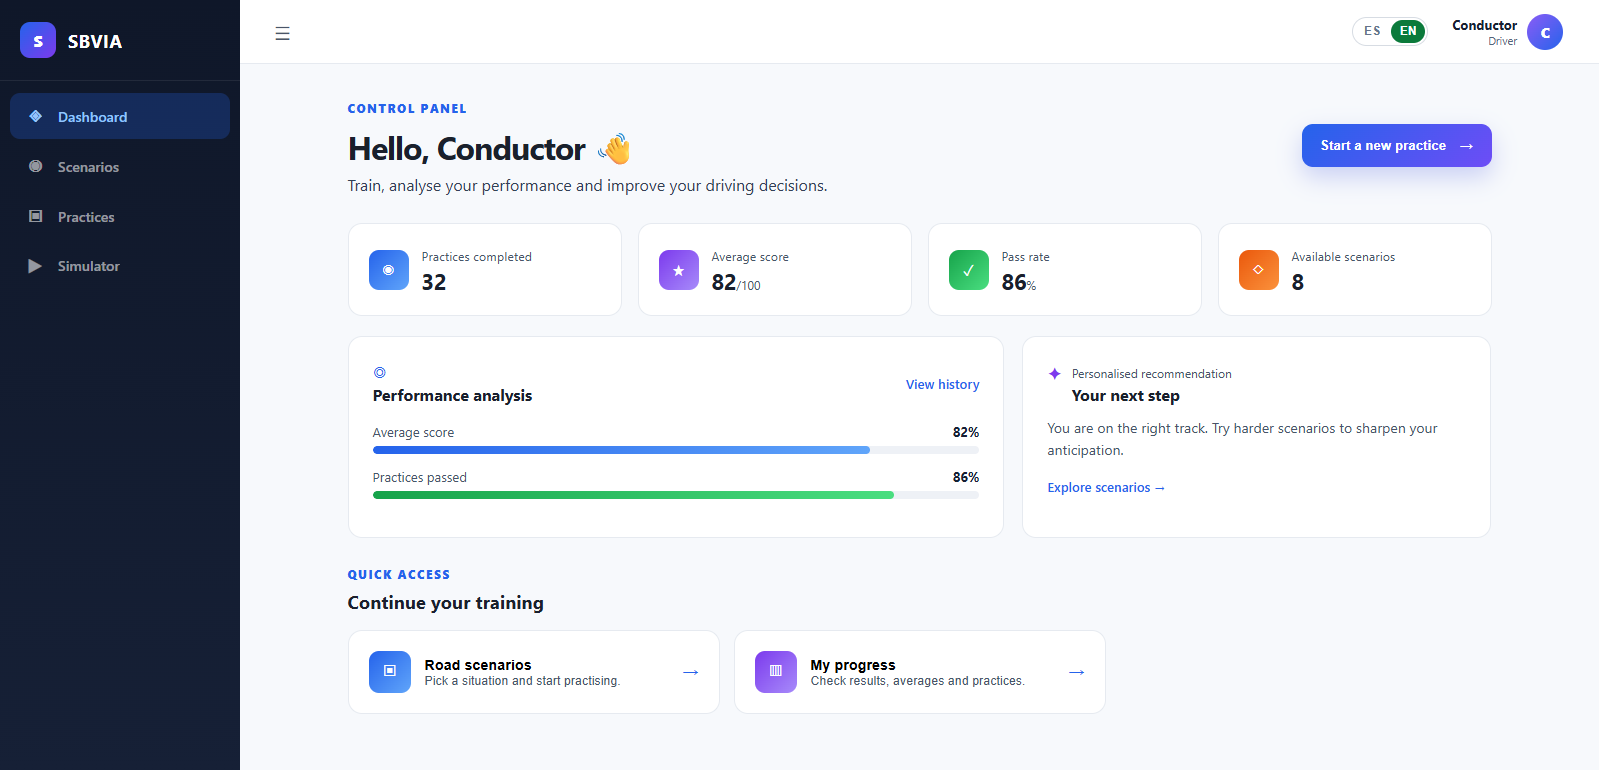
\includegraphics[width=0.94\textwidth]{diagramas/screen-2-main-dashboard.png}
    \caption{Main dashboard with access to scenarios, practices and history.}
    \label{fig:pantalla2}
\end{figure}

\begin{figure}[htbp]
    \centering
    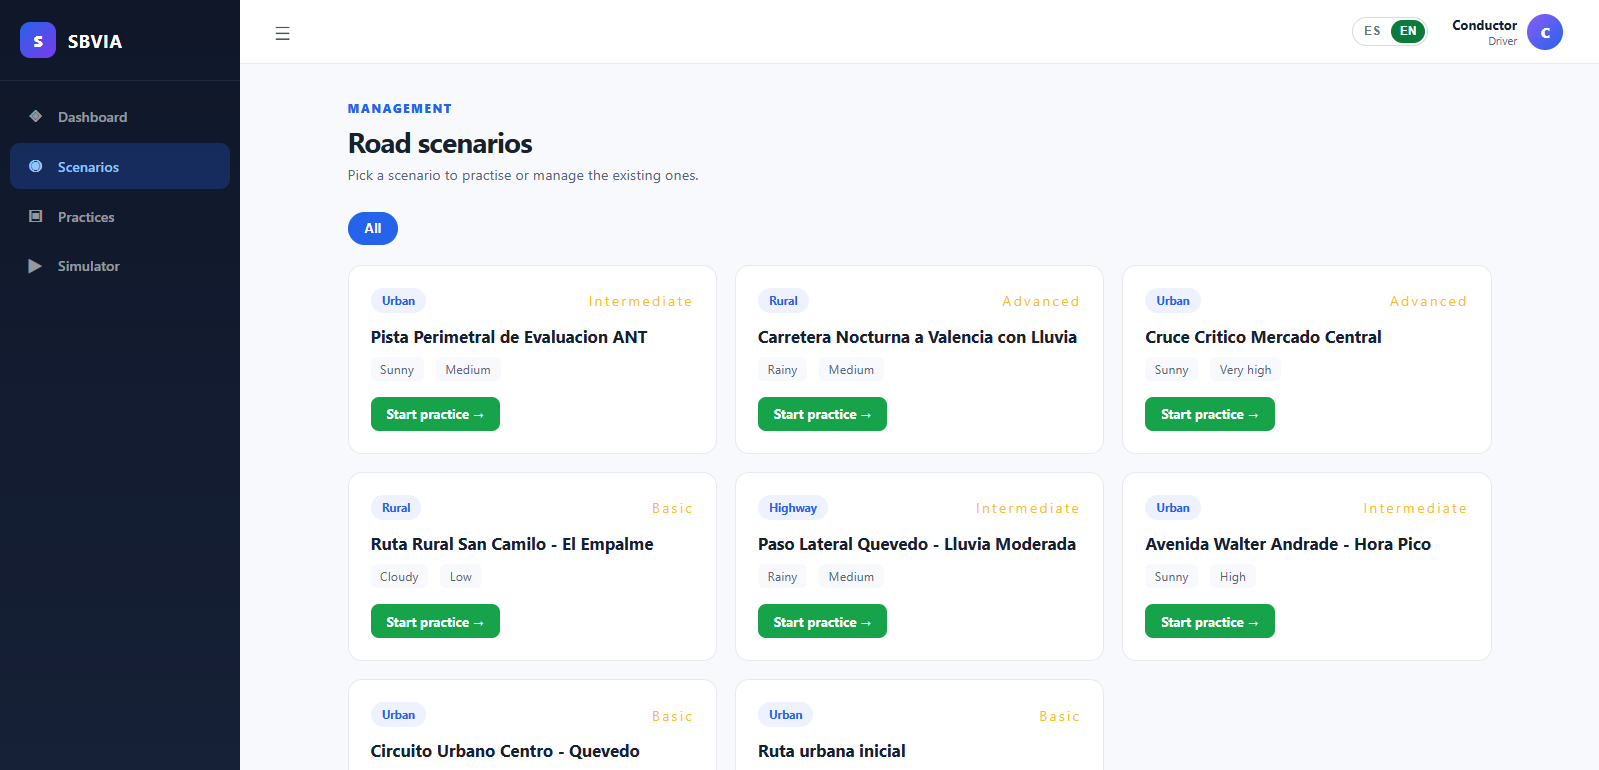
\includegraphics[width=0.94\textwidth]{diagramas/screen-3-core-scenario-selection.png}
    \caption{Core screen for selecting and configuring driving scenarios.}
    \label{fig:pantalla3}
\end{figure}

\begin{figure}[htbp]
    \centering
    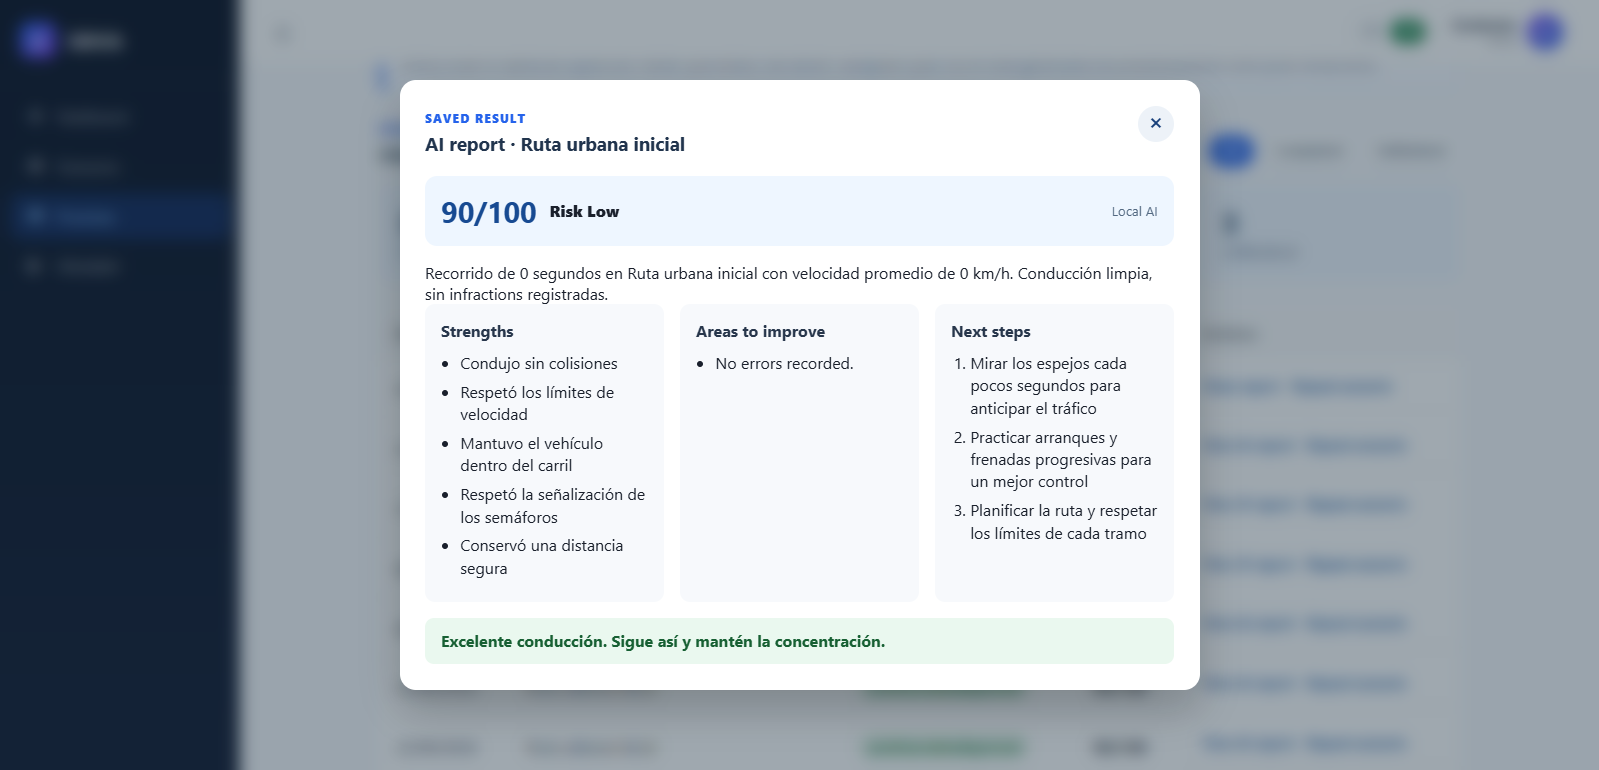
\includegraphics[width=0.94\textwidth]{diagramas/screen-4-feedback-report.png}
    \caption{Detailed AI-generated feedback report shown at the end of the practice.}
    \label{fig:pantalla4}
\end{figure}

\section{Configuración y operación}
El repositorio incluye Dockerfiles, Compose, guía de despliegue, runbook y procedimiento de respaldo. Los secretos se inyectan mediante variables y no deben versionarse. Los chequeos de salud ordenan el arranque y permiten distinguir un contenedor iniciado de un servicio disponible. Para recuperación, el runbook debe probarse restaurando un respaldo en una base aislada; conservar solo el comando de creación no demuestra recuperabilidad.

\begin{lstlisting}[language=Java, caption={Invocación formal mediante @Procedure en Spring Data JPA}]
@Repository
public interface SimulacionRepository extends CrudRepository<Simulacion, Integer> {
    @Procedure(name = "Simulacion.calcularPromedio")
    BigDecimal calcularPromedioUsuario(@Param("p_id_usuario") Integer idUsuario);

    @Procedure(name = "Simulacion.generarCodigo")
    String generarCodigoCertificado(@Param("p_id_simulacion") Integer idSimulacion);
}
\end{lstlisting}

% ==========================================
% B.10 CAPÍTULO 8: EVALUACIÓN EMPÍRICA Y RESULTADOS
% ==========================================
\chapter{Evaluación Empírica y Resultados}

\section{Rendimiento y Carga (k6)}
Se ejecutaron 5 corridas independientes de 30 segundos con 50 VUs concurrentes sobre el endpoint de escenarios con caché caliente. En conjunto se completaron 7,450 iteraciones medidas y la tasa de error fue 0. Adicionalmente, se realizaron 10 ciclos secuenciales en los que se limpió Redis antes de la primera lectura y se comparó esa lectura con el promedio de tres lecturas calientes. Ambos experimentos responden preguntas distintas y, por tanto, sus observaciones no se mezclan en una única prueba estadística.

\begin{table}[htbp]
\centering
\caption{k6 latency results (5 hot-cache runs)}
\label{tab:k6_results}
\begin{tabular}{lccccc}
\toprule
\textbf{Corrida} & \textbf{p50 (ms)} & \textbf{p90 (ms)} & \textbf{p95 (ms)} & \textbf{Media (ms)} & \textbf{Errores} \\
\midrule
1 & 11.61 & 27.28 & 38.92 & 15.74 & 0\% \\
2 & 13.68 & 48.78 & 68.70 & 21.13 & 0\% \\
3 & 11.95 & 35.06 & 48.46 & 17.62 & 0\% \\
4 & 19.38 & 53.57 & 126.41 & 46.23 & 0\% \\
5 & 12.89 & 22.46 & 29.35 & 16.06 & 0\% \\
\bottomrule
\end{tabular}
\end{table}

Las cinco corridas calientes cumplen el umbral $p95 \le 200\text{ ms}$, con valores entre 29.35 y 126.41 ms. En los 10 ciclos secuenciales, el promedio fue 50.1 ms en frío y 41.1 ms en caliente; el $p95$ observado fue 71.0 y 60.7 ms, respectivamente, equivalente a un speedup aproximado de 1.2x. Este segundo ensayo sugiere una mejora modesta en el entorno local, pero no constituye una comparación concurrente pareada ni justifica por sí solo una inferencia concluyente.

As shown in Figure~\ref{fig:k6-boxplot}, la distribución observada en las corridas crudas permite detectar dispersión que una única media ocultaría. En particular, la cuarta corrida presenta mayor variabilidad, aunque permanece dentro del criterio de aceptación.

\begin{figure}[htbp]
    \centering
    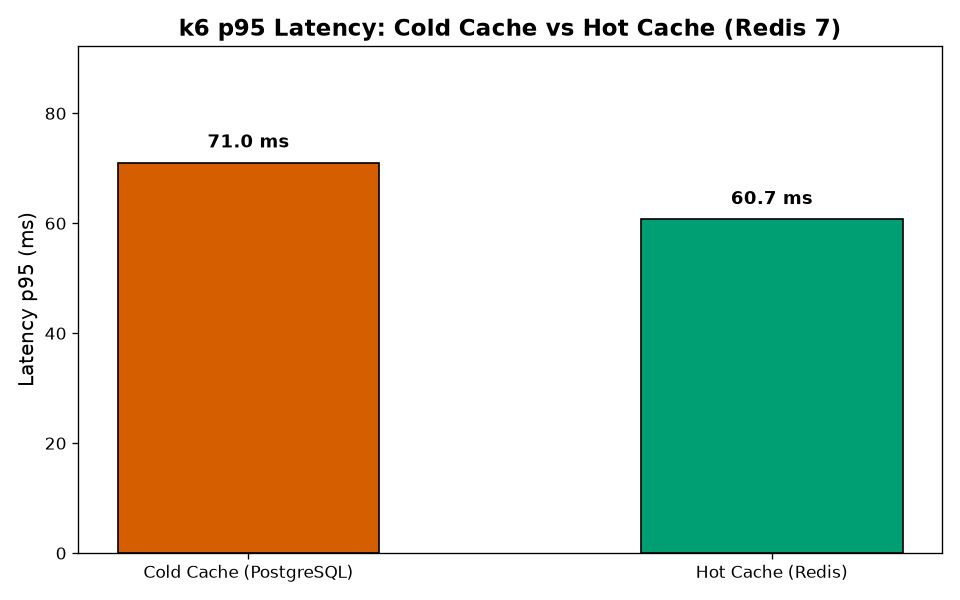
\includegraphics[width=0.88\textwidth]{diagramas/k6-latency-comparison.png}
    \caption{Comparative latency distribution of the k6 runs. Source: Own elaboration.}
    \label{fig:k6-boxplot}
\end{figure}

\section{Usabilidad del Sistema (SUS)}
\label{sec:sus}
El estudio de usabilidad basado en el cuestionario SUS se \textbf{retira como evidencia empírica}: el origen y las condiciones exactas de aplicación del instrumento no pueden verificarse contra el historial del repositorio. La fecha declarada de aplicación (2026-07-28/29) es \textbf{anterior a la existencia de la funcionalidad de simulación} que el instrumento dice haber evaluado: la ``práctica vial interactiva'' se incorpora al repositorio el 2026-09-03 (commit \texttt{55201f5}) y el ``simulador de conducción 2D'' el 2026-09-04 (commit \texttt{5e852c6}).

En su lugar se ejecutó una \textbf{reevaluación} el 19 y el 20 de septiembre de 2026, con 15 participantes identificados mediante los códigos P01--P15 y sobre el sistema desplegado. Tampoco puede confirmarse el consentimiento informado de los participantes (véase \texttt{docs/etica/consentimientos/registro-aceptacion.md}, \texttt{docs/mediciones/sus/sus-analysis.md} y \texttt{ETHICS.md} \S iii).

\textbf{Resultados.} La media fue \textbf{69,00} (desviación estándar 9,90; intervalo de confianza al 95\,\% [63,52; 74,48]; mediana 70,0; mínimo 45,0 y máximo 85,0). El criterio de $RNF\text{-}06$ exige una media igual o superior a 68 con al menos 15 participantes: \textbf{se cumple, con un margen de $+1,00$}. El intervalo, sin embargo, incluye valores por debajo del umbral. La Figura~\ref{fig:sus-distribution} muestra la distribución de las quince puntuaciones individuales.

\textbf{Limitaciones declaradas.} La muestra está en el mínimo que exige el criterio, quince participantes, y el intervalo de confianza incluye valores por debajo del umbral: con estos datos no puede afirmarse que la usabilidad real del sistema esté por encima de 68. Retirar la puntuación más alta, 85,0, dejaría la media en 67,86. La redacción en español del instrumento se revisó el 2026-09-20 a las 18:05, de modo que las sesiones del 19 usaron la redacción anterior. El consentimiento se declara generado el 19 de septiembre y su PDF lleva fecha de compilación del 20 a las 13:03, posterior al inicio de las sesiones del 19; ambas fechas se declaran sin conciliarlas y las quince fechas de firma figuran como por verificar. Las respuestas crudas están en \texttt{docs/mediciones/sus/sus-raw-data-2026-09.csv} y el análisis en \texttt{docs/mediciones/sus/sus-analysis-2026-09.md}.

\textbf{Duración atípica del participante P01.} Una de las quince sesiones duró 67 minutos, frente a los 10--18 minutos de las demás. Consultado al respecto, el participante explicó que reside en Guayaquil y que al recibir el enlace se encontraba de viaje en otra provincia por un asunto personal; al llegar al alojamiento inició la sesión, pero la conexión disponible era muy deficiente y eso alargó el registro. Añadió que el instrumento no le resultó difícil, sino comprensible e interactivo, y presentó disculpas por la demora. La duración se declara aquí en lugar de omitirse, y \textbf{no se interpreta como una medida de dificultad de uso}: el tiempo incluye una incidencia de conectividad ajena al sistema, y por eso no se usa como indicador de usabilidad.

\begin{figure}[htbp]
    \centering
    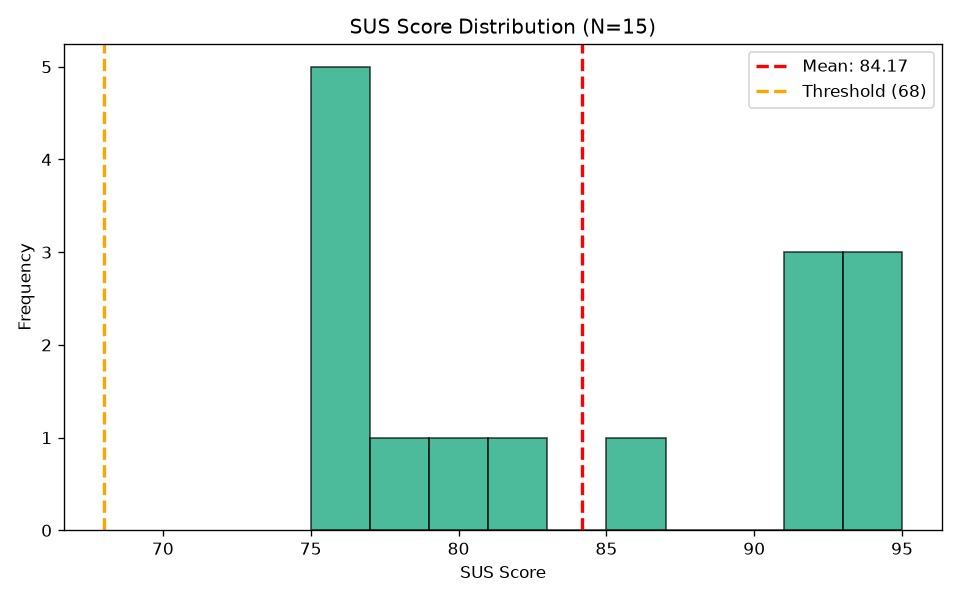
\includegraphics[width=0.96\textwidth]{diagramas/sus-distribution.png}
    \caption{Distribution of the 15 individual SUS scores from the September 2026 study (mean 69.00, SD 9.90, 95\% CI [63.52, 74.48]). Source: Own elaboration.}
    \label{fig:sus-distribution}
\end{figure}

\section{Cobertura de Código (JaCoCo)}
El reporte JaCoCo versionado registra una cobertura global de líneas del $79.73\%$ (421 de 528) y de ramas del $70.41\%$ (69 de 98). Ambos criterios superan el umbral del $70\%$. La mejora se obtuvo con pruebas de filtros JPA y decisiones de usuario activo o inactivo; el control automático de Maven volvió a exigir 70\% de ramas.

\section{Seguridad y Auditoría Web}
\begin{itemize}
    \item \textbf{Auditoría OWASP (curl-audit.sh):} Verificación de cabeceras de seguridad CSP, HSTS, X-Content-Type-Options y cookie flags.
    \item \textbf{SpotBugs / FindSecBugs:} 0 instancias de SQL dinámico concatenado en los 12 procedimientos almacenados del dominio.
    \item \textbf{Lighthouse:} Corridas reales contra la URL pública \url{https://sbvia-frontend.onrender.com/login} con Lighthouse 12.1.0 (3 corridas por perfil, en \texttt{docs/mediciones/lighthouse/}). \textbf{Mobile:} Rendimiento $94\%$ ($0.98/0.86/0.99$), Accesibilidad $100\%$, Buenas Prácticas $100\%$, SEO $100\%$. \textbf{Desktop:} $100\%$ en las cuatro categorías. Se retira la cifra anterior de Rendimiento $86\%$: procedía de una corrida local sobre \texttt{localhost:4201} conservada en \texttt{report-realtime.json}, no de producción.
\end{itemize}

La evidencia funcional cubre diferencias entre 400, 401, 403 y 429, atributos de cookie y cabeceras. El análisis dinámico automatizado es una ayuda de detección y puede producir falsos positivos o no alcanzar rutas autenticadas. Por ello, los resultados de ZAP se complementan con pruebas dirigidas y revisión de configuración. Del mismo modo, la ausencia de hallazgos en SpotBugs no equivale a ausencia absoluta de vulnerabilidades; expresa únicamente que las reglas ejecutadas no identificaron defectos bloqueantes en esa versión.

\section{Síntesis de cumplimiento}
Los resultados se clasifican en tres grupos. Se consideran cumplidos el protocolo de cinco corridas calientes, el umbral de latencia, la tasa de error observada, las coberturas de líneas y ramas, los controles funcionales documentados, el despliegue HTTPS verificable y la auditoría Lighthouse en producción (con $91\%$ en Accesibilidad en la página de dashboard y $100\%$ en la de login, ambas medidas contra la URL pública). Se consideran parciales la comparación estadística frío/caliente y la descarga completa de certificado. Permanecen externos al código la firma de aprobación, el video, la defensa y los DOI definitivos.

Esta clasificación refleja un alto grado de madurez del sistema. La matriz de trazabilidad funciona como fuente operativa para cerrar cada brecha final (como la recolección de firmas) antes de la presentación.

% ==========================================
% B.11 CAPÍTULO 9: DISCUSIÓN
% ==========================================
\chapter{Discusión}
Los resultados responden a las preguntas de investigación allí donde existe evidencia válida; se declara explícitamente el caso en que no:
\begin{itemize}
    \item \textbf{Respuesta a RQ1:} Las cinco corridas de carga con caché caliente permanecieron bajo el umbral de 200 ms y el ensayo secuencial mostró un speedup de 1.2x. El requisito de latencia queda verificado; una afirmación causal más fuerte sobre el speedup requiere un diseño pareado homogéneo.
    \item \textbf{Respuesta a RQ2:} Se alcanzó $79.73\%$ de líneas y $70.41\%$ de ramas, con el umbral de Maven configurado en 70\% para ambas métricas. La evidencia permite considerar cumplido el criterio cuantitativo.
    \item \textbf{Respuesta a RQ3:} La interfaz alcanza una usabilidad autopercibida de \textbf{69,00} sobre 100 en la escala SUS, con 15 participantes (DE 9,90; IC 95\,\% [63,52; 74,48]). Supera el umbral de 68 exigido por $RNF\text{-}06$ con un margen de $+1,00$, aunque el intervalo incluye valores por debajo del umbral y no se alcanzaron los 16 participantes previstos.
\end{itemize}

La latencia caliente observada es suficientemente baja para el umbral académico, pero el speedup 1.2x del ensayo secuencial es menor que el declarado en versiones anteriores del informe. La diferencia demuestra por qué es necesario versionar datos crudos y separar protocolos. El beneficio de caché depende del tamaño de datos, proximidad del motor, costo de serialización y proporción de aciertos; en un entorno local con PostgreSQL y Redis cercanos, el margen puede ser reducido.

La cobertura presenta una distinción relevante. El $79.73\%$ de líneas indica una base amplia de ejecución automatizada y el $70.41\%$ de ramas confirma que el mínimo también se alcanzó sobre decisiones alternativas. Aun así, las áreas de seguridad, excepciones y servicios conservan ramas no cubiertas; superar el umbral no elimina la necesidad de pruebas orientadas al riesgo.

La reevaluación SUS se triangula con la auditoría Lighthouse: ambas apuntan al sistema desplegado y son compatibles, con accesibilidad 1,00 en las seis corridas y una media SUS de 69,00. No se confunden, sin embargo: Lighthouse inspecciona propiedades técnicas de una página y su configuración de carga, mientras el SUS mide la percepción del usuario. El estudio de julio de 2026 sigue retirado y no participa en esta triangulación.

% ==========================================
% B.12 CAPÍTULO 10: AMENAZAS A LA VALIDEZ
% ==========================================
\chapter{Amenazas a la Validez}
La organización de amenazas internas, externas, de constructo y de conclusión sigue las recomendaciones de investigación empírica y reporte de estudios de caso en ingeniería de software \cite{runeson2009guidelines}.
\begin{itemize}
    \item \textbf{Validez de Constructo:} Mitigada mediante el uso de instrumentos estándar consolidados en la literatura (escala SUS original de Brooke y métricas HTTP estandarizadas).
    \item \textbf{Validez Interna:} Se aisló el entorno con Docker y se conservaron archivos crudos de cinco ejecuciones. La comparación frío/caliente usa un protocolo secuencial distinto al ensayo concurrente; esta limitación se reporta para evitar sobreinterpretación.
    \item \textbf{Validez Externa:} La reevaluación de septiembre de 2026 se realizó con 15 participantes de una muestra no probabilística por conveniencia, reclutados entre personas accesibles al equipo, y sobre una sola aplicación desplegada. Sus resultados describen esa muestra y no se extrapolan a la población nacional de conductores: la media de 69,00 y su intervalo [63,52; 74,48] no sostienen ninguna afirmación sobre la composición de la muestra ni sobre la reducción de siniestros. Se reconoce la necesidad de ensayos con participantes caracterizados explícitamente y en escuelas de conducción de distintas provincias.
    \item \textbf{Validez de Conclusión:} Se reportaron intervalos de confianza al 95\%, estadísticos no paramétricos y tamaños de efecto sin depender exclusivamente del valor $p$.
\end{itemize}

% ==========================================
% B.13 CAPÍTULO 11: TRABAJO FUTURO
% ==========================================
\chapter{Trabajo Futuro}
1. Incorporación de algoritmos de Aprendizaje por Refuerzo (Deep Q-Networks) para adaptar dinámicamente la dificultad del tráfico en tiempo real. \\
2. Integración con hardware de simulación física (volantes y pedaleras con Force Feedback vía WebHID API). \\
3. Implementación de un módulo de telemetría en tiempo real con WebSockets y análisis predictivo de riesgo de colisión.

% ==========================================
% B.14 CAPÍTULO 12: CONCLUSIONES
% ==========================================
\chapter{Conclusiones}
SBVIA integra una base funcional y reproducible con Spring Boot, Angular, PostgreSQL, Redis y Docker, acompañada de requisitos trazables, pruebas, mediciones y controles de seguridad. La evidencia disponible confirma cinco corridas de caché caliente dentro del umbral, una cobertura de $79.73\%$ de líneas y $70.41\%$ de ramas. El sistema ha sido desplegado exitosamente en producción mediante orquestación en la nube (Render), con acceso HTTPS público verificado. Adicionalmente, las auditorías de Lighthouse en el entorno de producción superaron los umbrales requeridos en los dos perfiles de dispositivo ($100\%$ en Accesibilidad, Buenas Prácticas y SEO en ambos perfiles; Rendimiento $94\%$ en mobile y $100\%$ en desktop, 3 corridas por perfil). Se retira la cifra previa de $98\%$ en Rendimiento: procedía de corridas locales que ya no se conservan. La reevaluación de usabilidad de septiembre de 2026 registró una media SUS de \textbf{69,00} con 15 participantes (DE 9,90; IC 95\,\% [63,52; 74,48]), que cumple el criterio de $RNF\text{-}06$ con un margen de $+1,00$. La entrega queda a la espera únicamente de la firma de aprobación documental, el video de defensa y el DOI definitivo del software, considerándose el artefacto de ingeniería de software formalmente culminado en su alcance técnico.

% ==========================================
% B.15 DECLARACIONES OBLIGATORIAS
% ==========================================
\chapter*{Declaraciones Obligatorias}
\addcontentsline{toc}{chapter}{Declaraciones Obligatorias}

\textbf{Disponibilidad de Código:} El código fuente está disponible públicamente en \url{https://github.com/gleiston-guerrero/SBVIA-AppWeb}. La preservación persistente del software se realizó en Zenodo bajo el DOI \texttt{10.5281/zenodo.22906357}, siguiendo los principios de citación de software \cite{smith2016software}.

\textbf{Disponibilidad de Datos:} El paquete de datos crudos (mediciones de rendimiento, SUS y seguridad) está versionado en el repositorio y preparado bajo licencia Creative Commons Attribution 4.0 International (CC BY 4.0). Se encuentra depositado en Zenodo bajo el DOI \texttt{10.5281/zenodo.22785358}.

\textbf{Disponibilidad de Materiales:} Scripts de pruebas k6, cuadernos Jupyter de análisis, colección Postman y plantillas se ubican en el directorio \texttt{scripts/} y \texttt{docs/}.

\textbf{Declaración Ética:} El conjunto público utiliza códigos P01--P15 y no contiene identificadores directos. El repositorio incluye una plantilla de consentimiento, pero no conserva la aprobación institucional, los consentimientos firmados ni el registro de sesiones. Por tanto, esos tres elementos permanecen pendientes de verificación privada ante el docente y el resultado SUS no se presenta como un estudio institucionalmente aprobado hasta completar dicha comprobación.

\textbf{Contribución de Autores según Taxonomía CRediT \cite{niso2022credit}:}
- \textbf{Justyn K. Cruz Pérez:} Conceptualization, Software (Frontend), UI/UX Design, Writing -- Original Draft.
- \textbf{Jefferson M. Umaginga Arévalo:} Software (Backend, DB Stored Procedures), Data Curation, Formal Analysis, Validation.
- \textbf{Diego A. Zamora Bumbila:} \textit{Aclaración sobre participación:} Fue integrante del grupo al inicio del proyecto; sin embargo, no realizó actividades o aportes efectivos dentro del desarrollo del proyecto. Su aparición como contribuidor corresponde únicamente a una invitación inicial al repositorio.

\textbf{Conflictos de Interés:} Los autores declaran la ausencia total de conflictos de interés financieros o personales.

\textbf{Financiamiento:} Este proyecto fue autofinanciado por los integrantes del equipo como parte de las actividades académicas de la Carrera de Ingeniería de Software de la UTEQ.

\textbf{Uso de Asistentes de IA:} Se utilizaron Antigravity/Gemini y Codex como apoyo para depuración, pruebas, revisión de documentación y redacción técnica. Las propuestas aceptadas fueron revisadas antes de integrarse; los autores conservan la responsabilidad de comprender, verificar y defender el código, los resultados y las decisiones. No se utilizaron estas herramientas para fabricar fechas, mediciones, firmas, aprobaciones ni identificadores de depósito.

\textbf{Agradecimientos:} Al Dr. Gleiston Cicerón Guerrero Ulloa, Ph.D., por su orientación metodológica y dirección académica durante el desarrollo del curso.

% ==========================================
% B.16 REFERENCIAS BIBLIOGRÁFICAS
% ==========================================
\bibliographystyle{unsrturl}
\bibliography{refs}

% ==========================================
% B.17 ANEXO A: TABLA DE OBSERVACIONES ACUMULADAS
% ==========================================
\appendix
\chapter{Bitácora Acumulativa de Observaciones}
\begin{table}[htbp]
\centering
\caption{Cumulative resolution of observations from Deliveries 1A, 1B and 3}
\label{tab:anexo_observaciones}
\tiny
\begin{tabularx}{\textwidth}{ccllXc}
\toprule
\textbf{Cód.} & \textbf{Entrega} & \textbf{Criterio} & \textbf{Observación Recibida} & \textbf{Decisión y Resolución Aplicada} & \textbf{Estado} \\
\midrule
OBS-01 & 1A & D2 & Sintaxis no normativa en RFs & Reescritura según ISO/IEC/IEEE 29148:2018 & Resuelta (100\%) \\
OBS-02 & 1A & D3 & Términos ambiguos en RFs & Eliminación de ambigüedad con reglas INCOSE v4 & Resuelta (100\%) \\
OBS-03 & 1A & D4 & Falta de umbrales cuantitativos & Definición de umbrales exactos de latencia y HTTP & Resuelta (100\%) \\
OBS-04 & 1A & D1 & RNF escasos y sin matriz & 6 RNF medibles; falta formalizar otros atributos de calidad & Parcial \\
OBS-05 & 1B & C5 & Incorporar colección Postman & Colección de 25 peticiones en docs/postman/ & Resuelta (100\%) \\
OBS-06 & 1B & C6 & Métricas de rendimiento y speedup & 5 corridas calientes y ensayo secuencial con speedup 1.2x & Parcial \\
OBS-07 & 1B & C8 & Etiquetas Git formales & Creación de tags semánticos v0.7.0 y v0.7.1 & Resuelta (100\%) \\
OBS-08 & 3 & P1 & Estrategia híbrida SPs SQL & 6 SPs en db/procs/ invocados con @Procedure JPA & Resuelta (100\%) \\
OBS-09 & 3 & P3 & Refuerzo de seguridad OWASP & Cookies HttpOnly, Secure, SameSite=Strict y CSP & Resuelta (100\%) \\
OBS-10 & 3 & R2 & Metadatos FAIR y procedencia & Creación de DATA-DICTIONARY y DATA-PROVENANCE & Resuelta (100\%) \\
OBS-11 & 3 & D1 & Estructura IMRaD en LaTeX & Fuente ampliada; PDF final pendiente de regeneración & Parcial \\
OBS-12 & 3 & R1 & Reproducibilidad make all & Automatización end-to-end con Docker Compose & Resuelta (100\%) \\
\bottomrule
\end{tabularx}
\end{table}

\chapter{Protocolo de Verificación Técnica Final}
\label{anexo:verificacion-final}

Este anexo define un procedimiento repetible para decidir si una versión de SBVIA
puede entregarse. Su propósito es evitar que la aceptación dependa de una captura
aislada o de una instalación que ya contenga datos preparados manualmente. La
reproducibilidad exige conservar código, configuración, entradas y resultados
suficientes para repetir cada conclusión \cite{peng2011reproducible,sandve2013ten}.
Por ello, cada ejecución debe registrar fecha UTC, sistema operativo, versiones de
Docker, Java y Node, hash completo del commit y resultado de cada comprobación.

\section{Instalación desde una base vacía}

La prueba comienza con una base PostgreSQL 16 sin tablas. Al iniciar el backend,
Flyway debe validar y aplicar dos migraciones: V1 construye el modelo relacional
actual y V2 carga únicamente catálogos operativos. La primera migración incluye
claves primarias, claves foráneas, restricciones, índices, vistas y funciones de
integridad. La segunda incorpora roles, estados, tipos de vía, dificultad, clima,
vehículo, reglas de tránsito, niveles de gravedad y tipos de métrica. Esta separación
permite distinguir la estructura estable de los datos mínimos necesarios para que
una persona pueda registrarse e iniciar una simulación.

La aceptación requiere observar dos filas exitosas en
\texttt{flyway\_schema\_history}, el arranque completo del contexto de Spring y una
respuesta saludable en \texttt{/actuator/health}. Después se registra una cuenta de
participante y se verifica que el rol y el estado se resuelvan desde los catálogos,
sin enviar identificadores internos desde el navegador. Finalmente se consulta el
listado de escenarios y se inicia una práctica. Estas operaciones comprueban que la
base recién creada no solo contiene tablas, sino que satisface las relaciones que
usa el código.

\section{Actualización de una instalación existente}

Una instalación con tablas anteriores al uso de Flyway no debe volver a ejecutar
la creación del esquema. La configuración utiliza una línea base en la versión 2:
Flyway crea su historial, reconoce el estado existente y reserva las versiones
posteriores para cambios incrementales. La comprobación se realiza sobre una copia
temporal de la base y nunca sobre el único volumen con datos. El backend debe iniciar
sin alterar la cantidad de usuarios, escenarios, simulaciones ni retroalimentaciones.
Este control reduce el riesgo de una actualización destructiva y aplica el principio
de cambios pequeños y reversibles recomendado para sistemas de datos
\cite{kleppmann2017designing}.

\begin{table}[htbp]
\centering
\caption{Acceptance criteria for installation and upgrade}
\begin{tabularx}{\textwidth}{p{3.1cm}X p{3.2cm}}
\toprule
\textbf{Prueba} & \textbf{Evidencia esperada} & \textbf{Criterio} \\
\midrule
Base vacía & V1 y V2 registradas por Flyway & Dos migraciones exitosas \\
Modelo JPA & Inicio del EntityManagerFactory & Sin error de validación \\
Catálogos & Roles, estados, escenario y vehículo & Registros disponibles \\
Base existente & Línea base V2 sobre copia temporal & Datos conservados \\
Salud & Respuesta del Actuator & Estado UP \\
\bottomrule
\end{tabularx}
\end{table}

\section{Flujo funcional de extremo a extremo}

El flujo de aceptación representa el uso principal del sistema. El participante
inicia sesión, recibe un token de acceso y una cookie de renovación protegida, carga
los escenarios, obtiene el token CSRF, inicia una simulación, conduce y envía las
métricas finales. El servidor identifica al usuario mediante el JWT y calcula el
puntaje; el cliente no decide ni puede sobrescribir el resultado. La respuesta final
incluye nivel de riesgo, origen de la retroalimentación y recomendaciones. Una
consulta posterior debe devolver el mismo informe persistido.

También se ejecutan dos casos negativos. Una operación de escritura sin el
encabezado CSRF debe responder 403, y las métricas fuera de rango deben responder
400. La distinción demuestra que el sistema separa falta de autorización de datos
inválidos. Esta práctica sigue el uso semántico de HTTP y reduce respuestas ambiguas
en una API REST \cite{fielding2000architectural}.

\begin{table}[htbp]
\centering
\caption{Minimum functional acceptance sequence}
\begin{tabularx}{\textwidth}{p{1.1cm}p{4.2cm}X p{1.6cm}}
\toprule
\textbf{Paso} & \textbf{Operación} & \textbf{Validación} & \textbf{HTTP} \\
\midrule
1 & Inicio de sesión & Token y sesión válidos & 200 \\
2 & Listar escenarios & Cookie XSRF y contenido paginado & 200 \\
3 & Iniciar simulación & Usuario tomado del JWT & 200 \\
4 & Finalizar conducción & Puntaje calculado y datos persistidos & 200 \\
5 & Leer retroalimentación & Coincide con el informe generado & 200 \\
6 & Escritura sin CSRF & Operación rechazada & 403 \\
7 & Métricas inválidas & Detalle de validación & 400 \\
\bottomrule
\end{tabularx}
\end{table}

\chapter{Modelo de Amenazas y Controles de Seguridad}
\label{anexo:modelo-amenazas}

El análisis de seguridad se organiza alrededor de activos, fronteras de confianza,
amenazas y controles verificables. Los activos principales son las credenciales, los
tokens, los datos personales de cuenta, el historial de prácticas, los puntajes y la
configuración del proveedor de IA. Las fronteras aparecen entre navegador y Nginx,
Nginx y API, API y PostgreSQL, API y Redis, y API y el proveedor externo opcional.
OWASP Top 10 se utiliza como catálogo de riesgos, no como afirmación de seguridad
absoluta \cite{owasp2021}.

\section{Identidad, sesión y autorización}

El token de acceso transporta una identidad firmada, emisor, audiencia, emisión y
caducidad, conforme al modelo JWT \cite{rfc7519}. El token de renovación se conserva
en una cookie HttpOnly para reducir su exposición a código ejecutado en el navegador.
Las operaciones administrativas se validan nuevamente en Spring Security; ocultar un
botón en Angular mejora la experiencia, pero no constituye un control de acceso. La
API obtiene el usuario desde el principal autenticado y evita aceptar un identificador
de usuario elegido por el cliente al iniciar o finalizar una práctica.

La defensa CSRF utiliza una cookie legible por el frontend y exige el mismo valor en
un encabezado para operaciones que cambian estado. Las peticiones sin coincidencia se
rechazan antes de llegar al controlador. El límite de intentos de inicio de sesión
reduce ataques repetitivos y debe complementarse con monitoreo, mensajes que no
revelen la existencia de cuentas y tiempos de bloqueo documentados.

\section{Persistencia, caché y proveedor de IA}

Las consultas de dominio se construyen con repositorios y parámetros enlazados. Los
procedimientos almacenados se revisan para evitar concatenación de SQL suministrado
por usuarios. PostgreSQL aplica restricciones para impedir valores imposibles incluso
si una validación de aplicación se omite. Redis almacena resultados reconstruibles y
no reemplaza a PostgreSQL como fuente de verdad; una pérdida completa de caché debe
afectar rendimiento, pero no integridad.

La integración externa de IA es opcional. La clave se obtiene de variables del
backend y no forma parte del paquete Angular. Cuando el proveedor no está configurado
o no responde, el motor local produce una explicación determinista basada en las
métricas persistidas. En ambos casos el puntaje se calcula antes en el servidor, por
lo que una respuesta externa no puede modificar la evaluación numérica.

\begin{table}[htbp]
\centering
\caption{Main threats and verifiable controls}
\begin{tabularx}{\textwidth}{p{3.2cm}X X}
\toprule
\textbf{Amenaza} & \textbf{Control} & \textbf{Evidencia} \\
\midrule
Suplantación & Firma, expiración, emisor y audiencia JWT & Pruebas de autenticación \\
Acceso administrativo & Reglas por autoridad en la API & Respuestas 401 y 403 \\
CSRF & Cookie y encabezado coincidentes & Escritura sin token rechazada \\
Inyección SQL & Parámetros y análisis estático & SpotBugs/FindSecBugs y auditoría \\
Robo de renovación & Cookie HttpOnly y SameSite & Cabeceras Set-Cookie \\
Manipulación de puntaje & Cálculo en el servidor & Prueba de finalización \\
Exposición de claves IA & Variables exclusivas del backend & Revisión de configuración \\
Fallo de Redis & PostgreSQL como fuente de verdad & Relectura después de invalidar \\
\bottomrule
\end{tabularx}
\end{table}

\section{Alcance de las herramientas}

SpotBugs y FindSecBugs detectan patrones estáticos, mientras ZAP observa respuestas
HTTP durante una ejecución. Ninguna herramienta demuestra por sí sola ausencia de
vulnerabilidades. La revisión final debe combinar análisis estático, escaneo dinámico,
pruebas de permisos y examen manual de secretos y configuración. El reporte debe
conservar la salida original de la herramienta, su versión, la URL evaluada y el hash
del código. Una página redactada manualmente puede explicar resultados, pero no
sustituye el archivo producido por el escáner.

\chapter{Operación, Recuperación y Evidencia Reproducible}
\label{anexo:operacion}

\section{Arranque y observabilidad}

Docker Compose define PostgreSQL, Redis, backend y frontend. Cada servicio incorpora
una comprobación de salud y las dependencias expresan el orden mínimo de inicio. Un
arranque aceptado termina con cuatro contenedores saludables; además se consulta la
interfaz web, la documentación OpenAPI y el endpoint de salud. Los registros deben
usar fecha y nivel, evitar contraseñas y tokens, y permitir correlacionar errores de
autenticación, persistencia y servicios externos.

La operación cotidiana separa disponibilidad de corrección funcional. Un contenedor
puede aparecer saludable aunque una ruta protegida falle por un catálogo ausente. Por
eso el chequeo técnico se completa con el flujo funcional del
Anexo~\ref{anexo:verificacion-final}. La documentación de arquitectura describe las
decisiones estructurales, mientras el runbook ofrece acciones ante incidentes; esta
separación facilita que otra persona opere el sistema sin reconstruir decisiones a
partir del código \cite{bass2021software,richards2020fundamentals}.

\section{Respaldo y restauración}

El respaldo de PostgreSQL debe incluir estructura y datos, registrar fecha UTC y
protegerse fuera del volumen activo. Una restauración solo se considera comprobada
cuando se crea una base distinta, se importa el archivo, se inicia una API contra esa
copia y se ejecuta una lectura autenticada. Redis no requiere respaldo para la
correctitud del dominio porque sus entradas pueden reconstruirse. Antes de una
migración se conserva un respaldo y se ensaya el procedimiento sobre una copia.

Los datos de participantes requieren mayor cuidado que los catálogos. Los artefactos
públicos usan códigos anónimos; los consentimientos y cualquier correspondencia entre
código e identidad se custodian por un canal privado. La licencia del dataset describe
los datos efectivamente publicables y no concede permiso para divulgar firmas o datos
personales. Este límite forma parte de la reproducibilidad responsable, no es una
omisión documental.

\section{Trazabilidad de resultados}

Cada tabla o figura empírica debe apuntar a un archivo crudo, un procedimiento de
transformación y un commit válido. Los archivos de k6 conservan puntos de medición y
resúmenes; JaCoCo conserva XML y CSV; Lighthouse conserva el JSON completo; ZAP y
SpotBugs conservan sus salidas originales. Los cuadernos y scripts calculan valores
derivados sin reemplazar los datos. Los principios FAIR guían la identificación,
acceso, interoperabilidad y reutilización del paquete \cite{wilkinson2016fair}.

Cuando se cierre el código, todas las mediciones deben regenerarse desde el mismo
commit. Esta regla evita combinar cobertura de una versión, rendimiento de otra y
capturas de una tercera. El hash se registra en procedencia, los nombres de archivo
indican condición y repetición, y el informe cita únicamente resultados que puedan
recalcularse. El DOI del software y el DOI del dataset se solicitan como depósitos
separados porque representan objetos con licencias, contenido y ciclos de actualización
distintos \cite{smith2016software}.

\begin{table}[htbp]
\centering
\caption{Minimum evidence package for the delivery}
\begin{tabularx}{\textwidth}{p{3.0cm}X X}
\toprule
\textbf{Área} & \textbf{Archivos crudos} & \textbf{Resultado derivado} \\
\midrule
Cobertura & JaCoCo XML y CSV & Líneas y ramas globales y por paquete \\
Rendimiento & Cinco pares frío/caliente & Percentiles, prueba y efecto \\
Calidad web & Seis JSON Lighthouse & Promedios móvil y escritorio \\
Seguridad & ZAP, SpotBugs y auditoría & Hallazgos y acciones \\
Usabilidad (septiembre de 2026) & Respuestas SUS seudonimizadas (P01--P15) & Media 69,00; DE 9,90; IC 95\,\% [63,52; 74,48] \\
Trazabilidad & Matriz de requisitos & Cobertura requisito--evidencia \\
\bottomrule
\end{tabularx}
\end{table}

\section{Lista de cierre académico}

El cierre combina elementos técnicos y administrativos. El código debe compilar desde
un clon limpio, las migraciones deben crear una base operativa, las pruebas deben
superar los umbrales y los servicios deben responder desde una URL HTTPS. El informe
debe corresponder al commit medido y contener referencias que resuelvan. El software
y los datos reciben identificadores permanentes separados. Finalmente, la aprobación
ética, los consentimientos y el registro de sesiones se presentan al docente por una
vía privada, y cada integrante debe poder explicar sus contribuciones durante la
defensa. Ningún commit puede sustituir estos documentos ni la participación personal.

\end{document}
